\documentclass[../main/main.tex]{subfiles}

\raggedbottom

\makeatletter
\renewcommand{\@chapapp}{M\'ecanique -- chapitre}
\makeatother

% \toggletrue{student}

\begin{document}
\setcounter{chapter}{0}

\chapter{Cin\'ematique du point}

La \textbf{cinématique} est l'étude du mouvement en soi. On ne s'intéresse pas
aux causes qui ont donné naissance au mouvement. Avant toute chose, introduisons
le vocabulaire autour de l'objet d'étude.

\section{Système et point matériel}
\subsection{Système}
\begin{bdefi}{Définition}
    \cswitch{white}{
    En mécanique, le \textbf{système} est l'objet ou groupe
    d'objets dont on souhaite étudier le mouvement.}\vspace{-12pt}
\end{bdefi}

La définition du système est primordiale et indispensable pour la mécanique. En
effet, l'étude du mouvement sera radicalement différente entre les systèmes
\{bille\} et \{bille+Terre\}. Il en sera de même en dynamique, où ce sont les
forces \textbf{extérieures} au système qui entrent en jeu, il faut donc définir
l'extérieur.

\subsection{Point matériel}

Dans la cadre de la mécanique du point, la forme de l'objet importe peu. Ainsi,
on choisira de suivre un point caractéristique du système, souvent son centre de
gravité. Celui-ci pourra être repéré dans l'espace et le temps par 3+1
coordonnées.

\begin{bdefi}{Définition}
    \cswitch{white}{
    Le point matériel est le point qui représente l'objet auquel on affecte
    toute la masse de l'objet considéré. Ce point, appelé souvent M et affecté
    de la masse $m$, est le point géométrique que l'on repère dans l'espace pour
    connaître son mouvement.}%\vspace{-10pt}
\end{bdefi}

\section{Description et paramétrage du mouvement}
\subsection{Notion de référentiel et relativité du mouvement}

Pour décrire le mouvement d'un objet, on doit~:
\begin{itemize}
    \item dire par \underline{rapport à quoi} il se déplace~: on définit alors
        une \textbf{origine}~;
    \item dire dans \underline{quelle direction} il se déplace~: on fixe alors
        un \textbf{repère} (système de coordonnées)~;
    \item dire sur \underline{quel intervalle de temps} il se déplace~: on
        définit un repère de temps.
\end{itemize}

\begin{bdefi}{Définition}
    Un \textbf{référentiel}, noté $\Rc$, est une référence permettant de décrire
    le mouvement d'un objet, constitué par~:
    \cswitch{white}{
    \begin{itemize}
        \item un repère permettant de décrire l'espace~;
        \item une horloge permettant de mesurer le temps.
    \end{itemize}
    }%\vspace{-10pt}
\end{bdefi}

Un mouvement est toujours relatif, et \textbf{la description d'un mouvement
dépend du référentiel}. Ainsi, on notera les grandeurs liées à un référentiel
\textit{via} l'indication de celui-ci en indice, précédé d'une barre oblique ou
verticale selon la taille de la grandeur~:
\[  \boxed{\vv{x}_{/\Rc}}
    \qou
    \boxed{\eval{\dv{\vv{x}}{t}}_{\Rc}}\]

\begin{rexem}{Exemple}
    \begin{itemize}
        \item Du point de vue de san voisin-e, læ passagær d'un train est
            immobile. Du point de vue du quai, cælui-ci est en translation.
        \item Du point de vue d'um cycliste, la valve de la roue est en rotation
            autour de l'axe de la roue. Selon um passant-e immobile, elle suit
            un mouvement de cycloïde. Son altitude atteint $0$ à chaque tour de
            roue.
            \begin{center}
                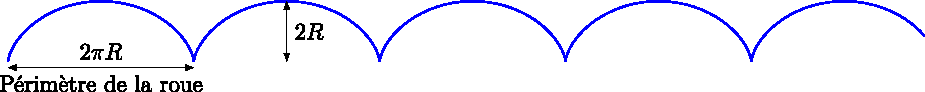
\includegraphics[width=\linewidth]{roue}
            \end{center}
    \end{itemize}
\end{rexem}

\begin{bror}{~}
    Nous resterons ici en mécanique \textbf{classique}, c'est-à-dire que les
    corps étudiés auront une vitesse très inférieure à celle de la lumière dans
    le vide. Ce faisant, les mesures de longueurs ou de durées seront
    \textbf{absolues} et indépendantes du référentiel. Ça n'est pas le cas en
    mécanique \textit{relativiste}.
\end{bror}

\subsection{Exemples de référentiels}

Le mouvement dépendant du référentiel, il faut choisir le référentiel adéquat
par rapport au mouvement que l'on souhaite étudier. Souvent, on choisit parmi
trois référentiels classiques dit \textit{galiléens}~: \bigbreak

\begin{itemize}

    \item Le référentiel \textbf{héliocentrique} est un référentiel dont le
        centre du repère est situé au centre du \textbf{Soleil}, et les trois
        axes du repère sont dirigés vers \textbf{trois étoiles lointaines
        considérées comme fixes}~; il est utile pour étudier les mouvements des
        planètes du système solaire.

    \item Le référentiel \textbf{géocentrique} est un référentiel centré au
        centre de la \textbf{Terre}, ses trois axes sont dirigés vers les trois
        \textbf{mêmes étoiles} que celles du référentiel de héliocentrique; il
        est utilise pour étudier les mouvements de satellites terrestres par
        exemple ;

    \item Les référentiels \textbf{terrestres} sont des référentiels liés à des
        objets fixes à la \textbf{surface} de la Terre~: lui est souvent associé
        un repère cartésien. Pour tous les mouvements qui se déroulent à la
        surface de la Terre, ce référentiel est approprié.
\end{itemize}


\subsection{Vecteur, base de projection et repère}
Pour décrire le mouvement d'un point dans l'espace, il est nécessaire d'utiliser
des vecteurs.
\begin{bdefi}{Définition}
    Un vecteur est un objet mathématique qui se dénote avec une flèche vers la
    droite au-dessus d'une lettre~: $\vec{\cdot}$, et ayant~:\smallbreak
    \cswitch{white}{
    \begin{minipage}{0.40\linewidth}
        \begin{itemize}
            \item Un \textbf{point d'application}~;
            \item Une \textbf{direction}~;
        \end{itemize}
    \end{minipage}
    \begin{minipage}{0.50\linewidth}
        \begin{itemize}
            \item Un \textbf{sens}~;
            \item Une distance appelée \textbf{norme}, notée $\norm{\vec{\cdot}}$.
        \end{itemize}
    \end{minipage}
    }
    \begin{framed}
        \centering
        \cswitch{white}{
        \textbf{Une} égalité de vecteurs donne \textbf{trois} égalités de
        scalaires, pour chaque direction de l'espace.
        }\vspace{-12pt}
    \end{framed}
\end{bdefi}

On utilise pour ça une \textbf{base orthonormée directe}, constituée de 3
vecteurs~:

\begin{minipage}{0.70\linewidth}
    \begin{itemize}
        \item \textbf{Ortho}~: les trois vecteurs de la base sont orthogonaux
            entre eux~;
        \item \textbf{Normée}~: la norme des trois vecteurs de la base est égale
            à 1. On dit qu'ils sont \textit{unitaires}~;
        \item \textbf{Directe}~: respecte la règle de la maint droite (chaque
            vecteur est égal au produit vectoriel des deux précédents) 
    \end{itemize}
\end{minipage}
\hfill
\begin{minipage}{0.20\linewidth}
    \begin{center}
        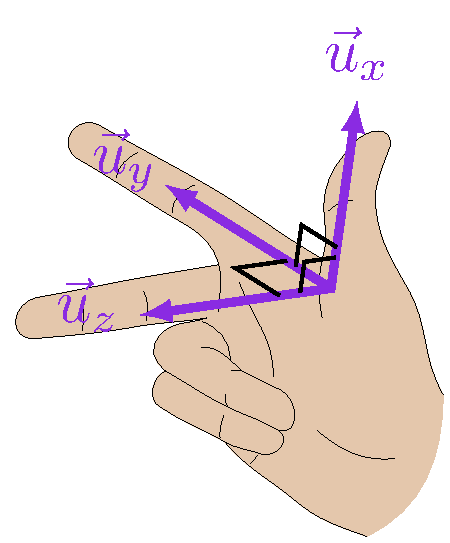
\includegraphics[width=\linewidth]{righthand}
    \end{center}
\end{minipage}
\hfill~

Les vecteurs de base n'ont \textbf{pas d'unité}. Ils définissent les trois
directions dans lesquelles le point M pourrait se mouvoir. Pour que le repérage
dans l'espace du point M soit optimal, on ajoute une origine O à la base~:
l'ensemble d'une \textbf{base} et d'une \textbf{origine} constituent un
\textbf{repère}. Le plus simple est le repère cartésien~:
\begin{bdefi}{Définition}
    \begin{minipage}{0.70\linewidth}
        \cswitch{white}{
        Le repère cartésien est constitué d'une origine O autour de laquelle
        sont définis trois vecteurs $\ux$, $\uy$ et $\uz$ de \textbf{direction
        constante dans le temps}. On trouve parfois la notation $\ex$, $\ey$,
        $\ez$.}
        \bigbreak
        Jusqu'à notifié autrement, ce sera notre repère de prédilection.
    \end{minipage}
    \hfill
    \begin{minipage}{0.25\linewidth}
        \begin{center}
            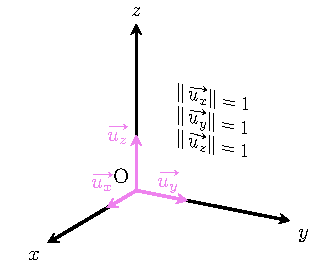
\includegraphics[width=\linewidth]{cart}
        \end{center}
    \end{minipage}
\end{bdefi}

\section{Position, vitesse et accélération}
\subsection{Position}
\subsubsection{Définition}

\begin{bdefi}{Définition}
    \begin{minipage}{0.70\linewidth}
        Le vecteur position noté $\OM(t)$ est le vecteur qui permet de repérer
        un point M d'un système dans l'espace et le temps par rapport à
        l'origine O d'un repère. \textbf{Il est homogène à une distance}.
        \smallbreak
        En coordonnées cartésiennes, la position d'un point M par rapport à
        l'origine O s'écrit~:
        \[\cswitch{white}{\OM(t) = x(t)\ux + y(t)\uy + z(t)\uy}\]
        et sa \textbf{norme} se calcule avec~:
        \[\cswitch{white}{\OMr = \norm{\OM} = \sqrt{x(t)^2 + y(t)^2 + z(t)^2}}\]
    \end{minipage}
    \hfill
    \begin{minipage}{0.29\linewidth}
        \begin{center}
            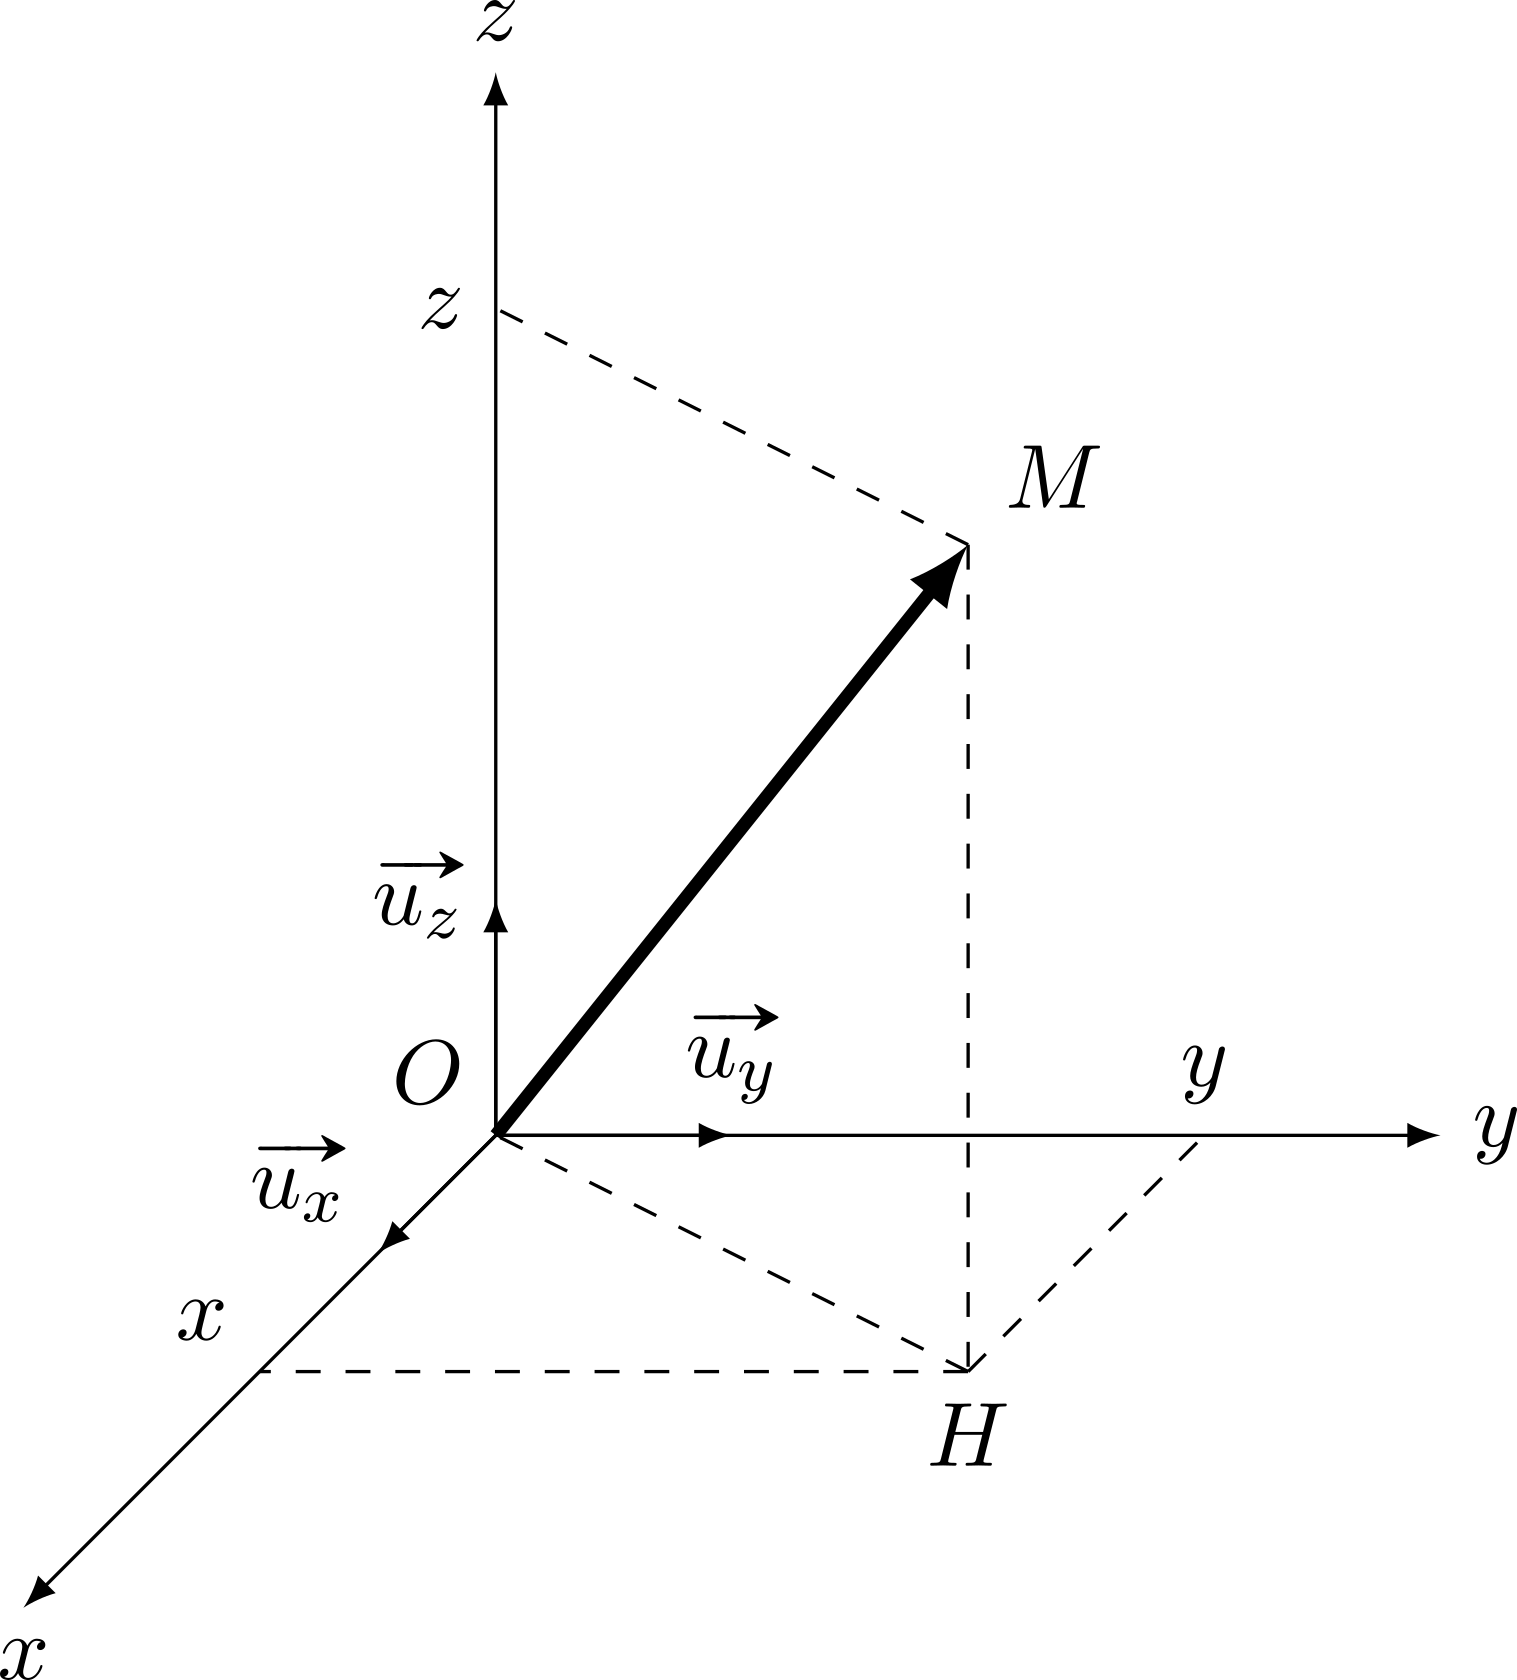
\includegraphics[width=\linewidth]{vec_pos}
        \end{center}
    \end{minipage}
\end{bdefi}

\subsubsection{Déplacement élémentaire}
\begin{bdefi}{Définition}
    Le \textbf{déplacement élémentaire} est le déplacement infiniment petit du
    point M pendant un temps infinitésimal $\dt$~:
    \[\cswitch{white}{\dd\OM = \OM(t+\dt)-\OM(t)}\]
    En coordonnées cartésiennes,
    \[\cswitch{white}{\boxed{\dd\OM = \dd{x}\ux + \dd{y}\uy + \dd{z}\uz}}\]
\end{bdefi}

\subsubsection{Équations horaires et trajectoire}
\begin{rdefi}{Déf.}
    Les \textbf{équations horaires} du mouvement sont les fonctions $x(t)$,
    $y(t)$ et $z(t)$ exprimées \textbf{explicitement} en fonction du temps $t$.
\end{rdefi}

En TP, on pourra étudier l'évolution de $x(t)$ et $y(t)$ dans différents cas~:
\bigbreak

\begin{minipage}{0.31\linewidth}
    \begin{itemize}
        \item chute dans le glycérol~:
    \end{itemize}
    \begin{center}
        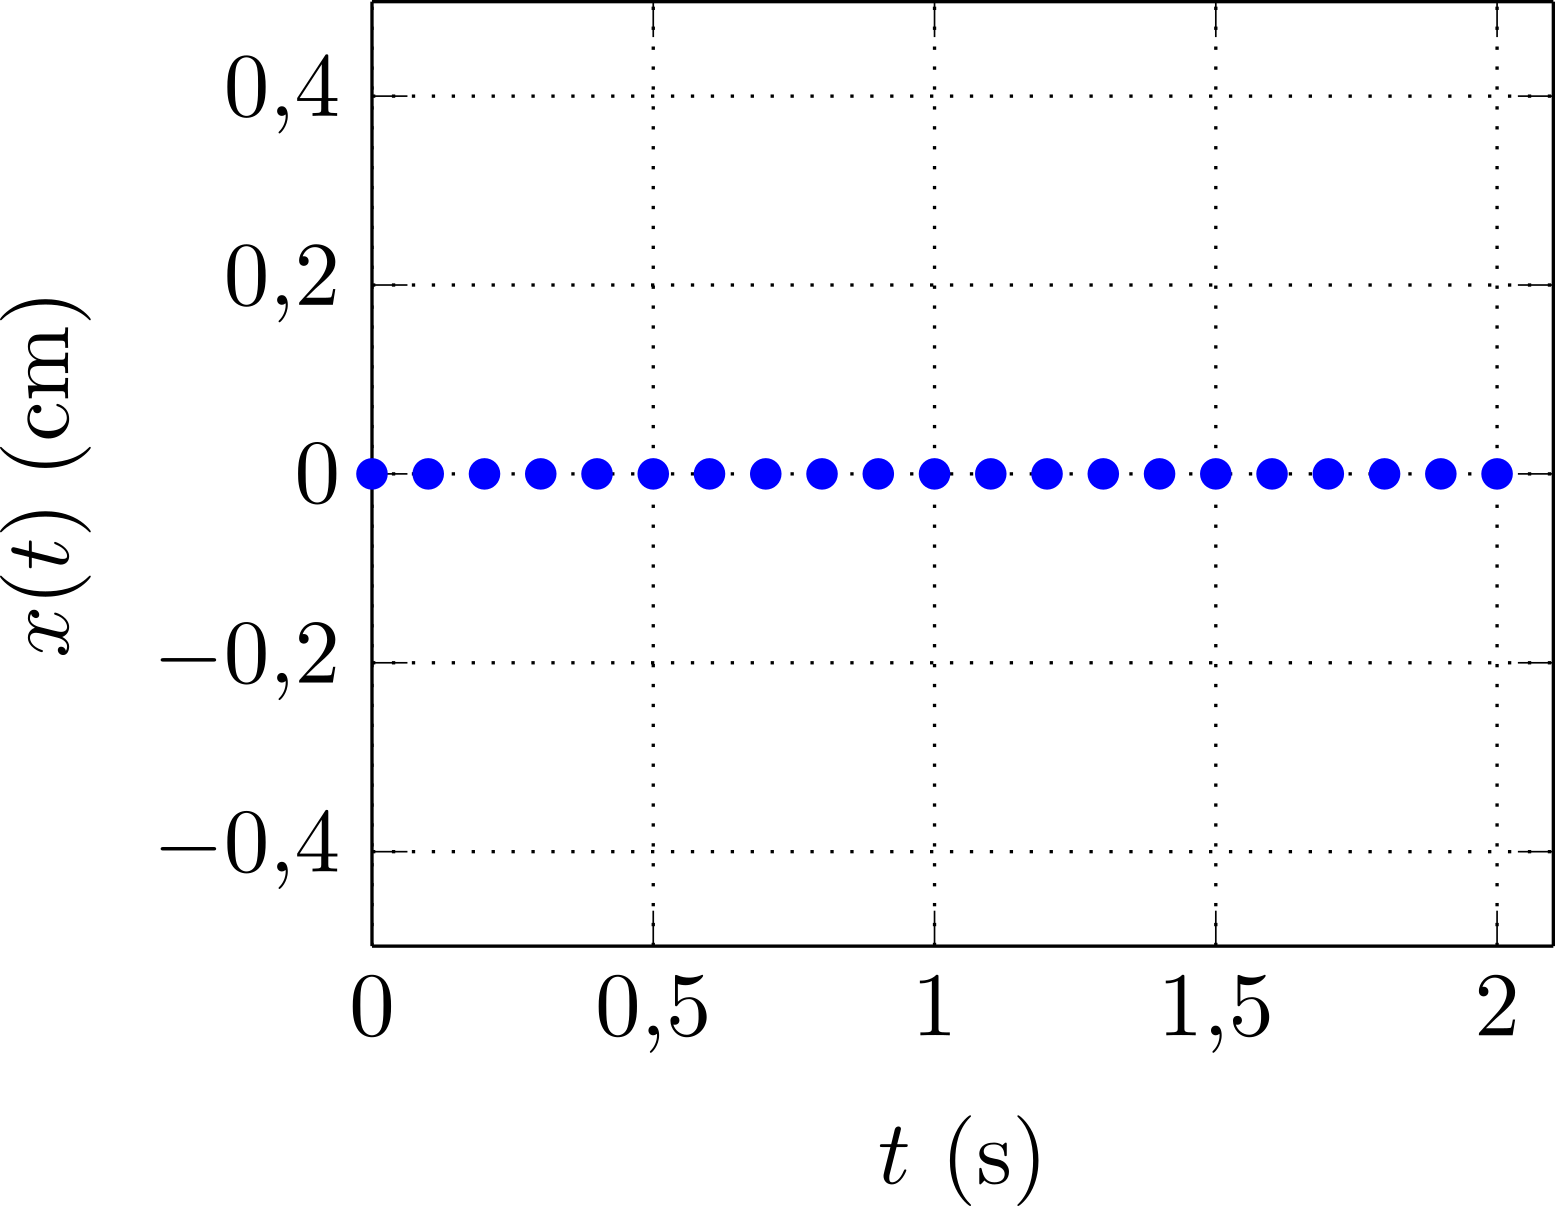
\includegraphics[width=\linewidth]{x_glyc}
        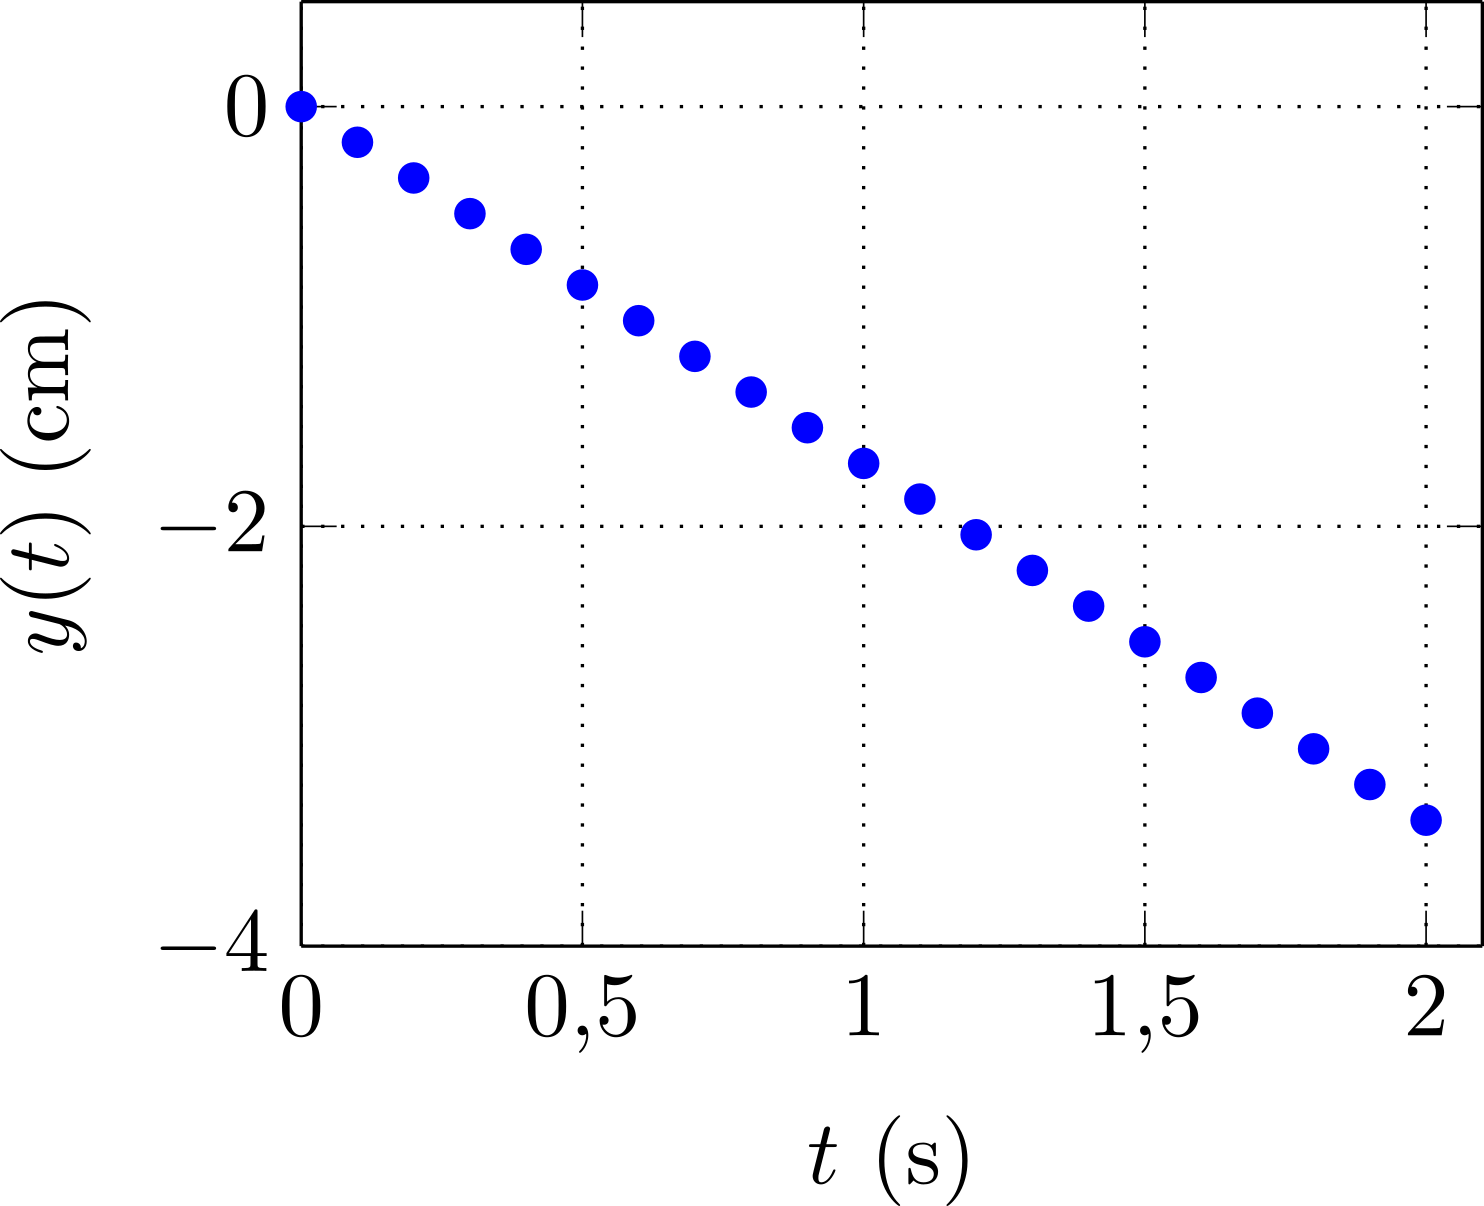
\includegraphics[width=\linewidth]{y_glyc}
    \end{center}
\end{minipage}
\hfill
\begin{minipage}{0.31\linewidth}
    \begin{itemize}
        \item chute libre sans vitesse initiale~:
    \end{itemize}
    \begin{center}
        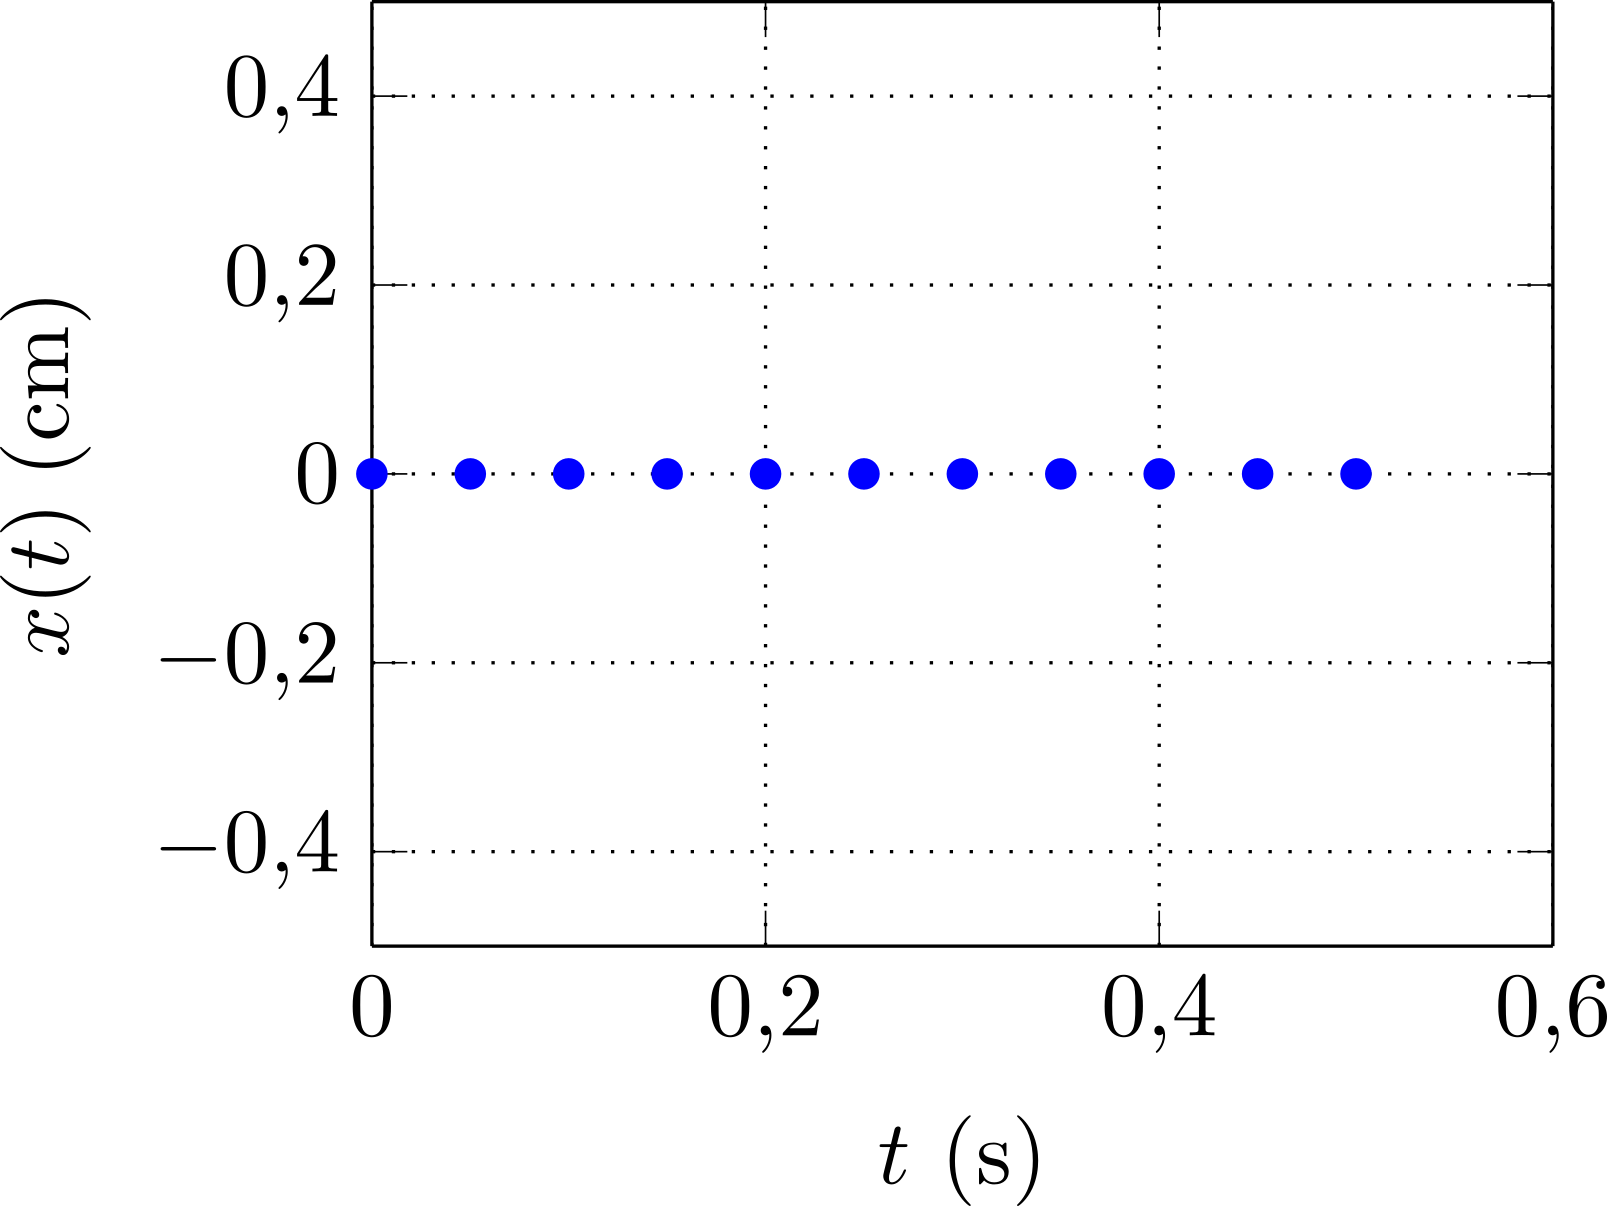
\includegraphics[width=\linewidth]{x_nov}
        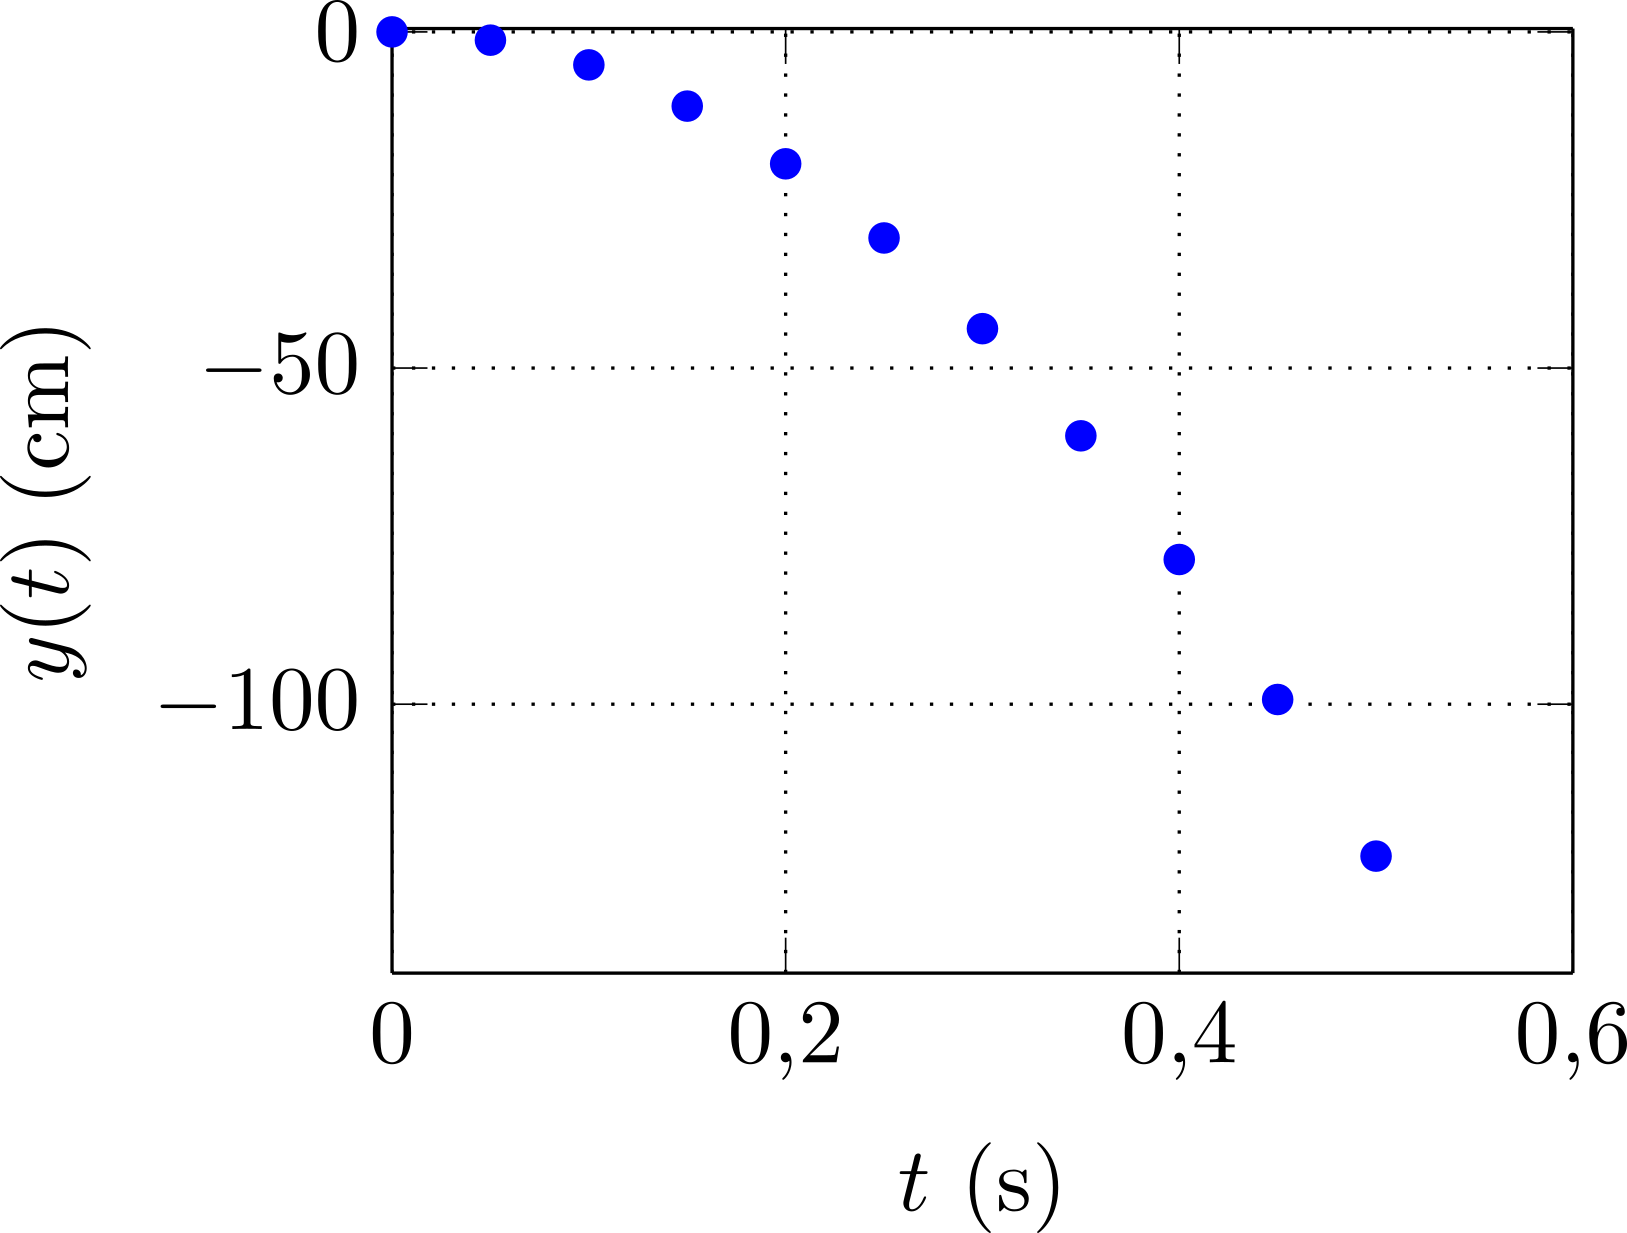
\includegraphics[width=\linewidth]{y_nov}
    \end{center}
\end{minipage}
\hfill
\begin{minipage}{0.31\linewidth}
    \begin{itemize}
        \item chute libre avec vitesse initiale~:
    \end{itemize}
    \begin{center}
        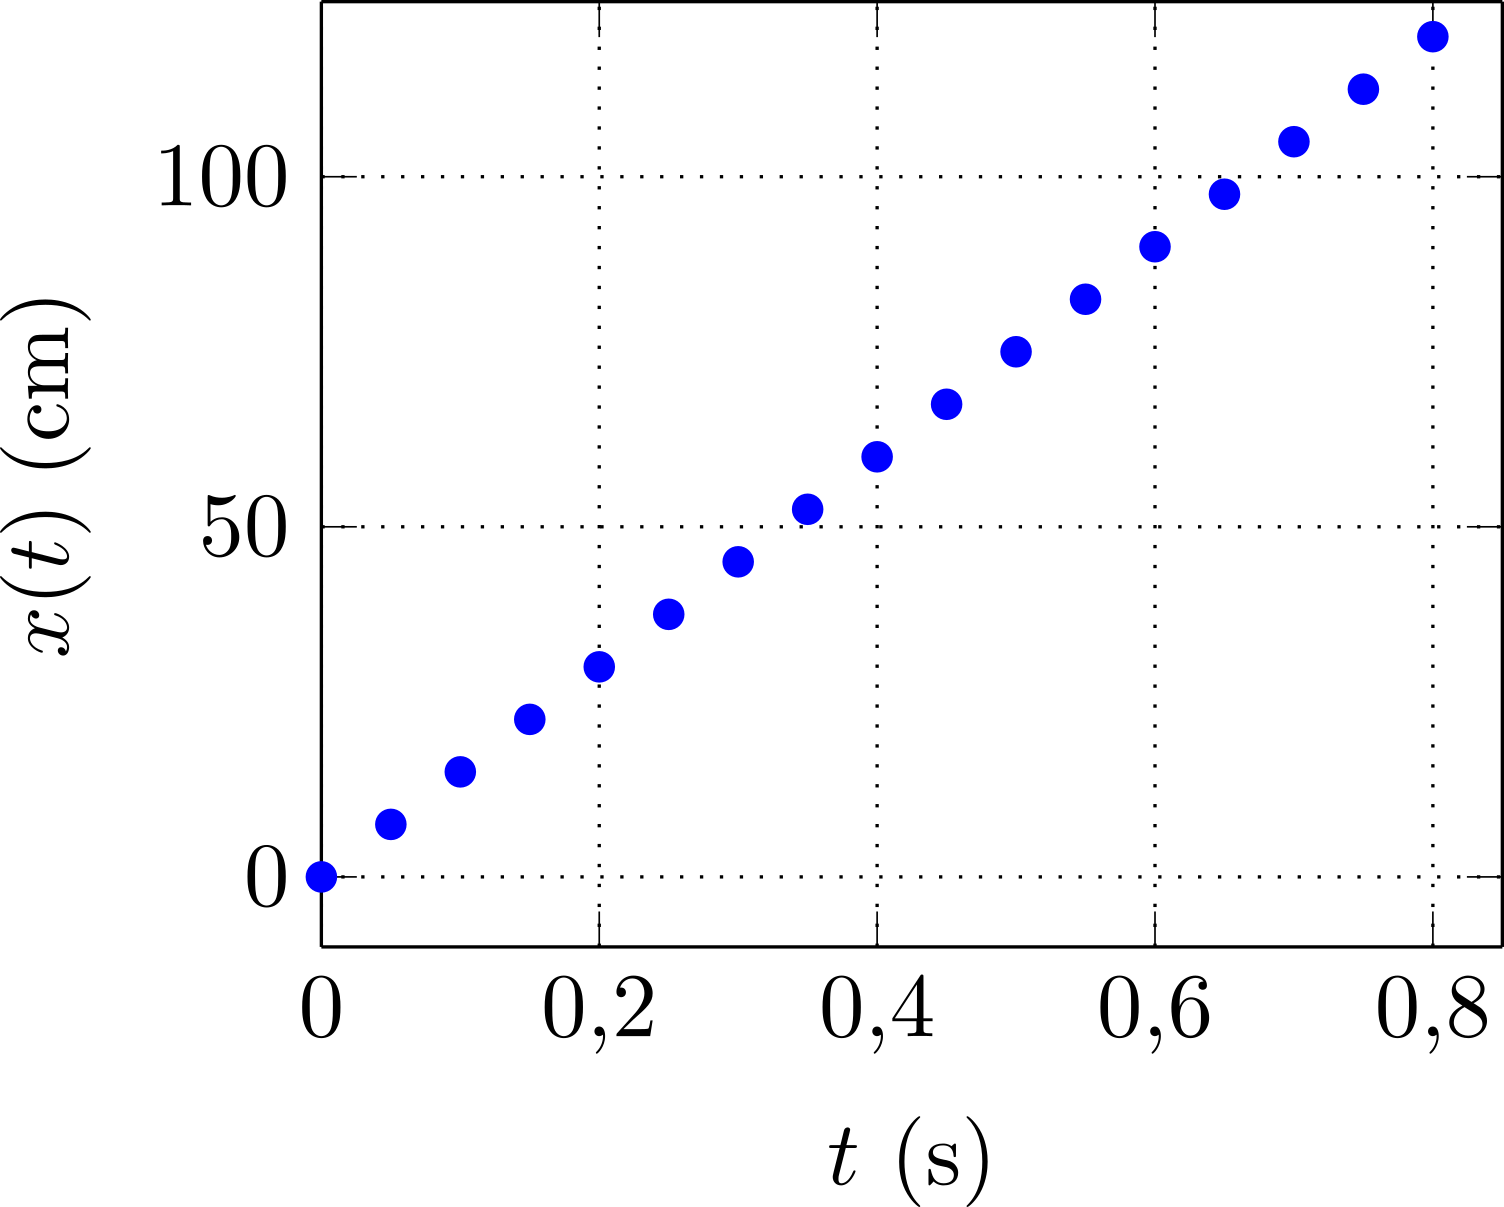
\includegraphics[width=\linewidth]{x_vo}
        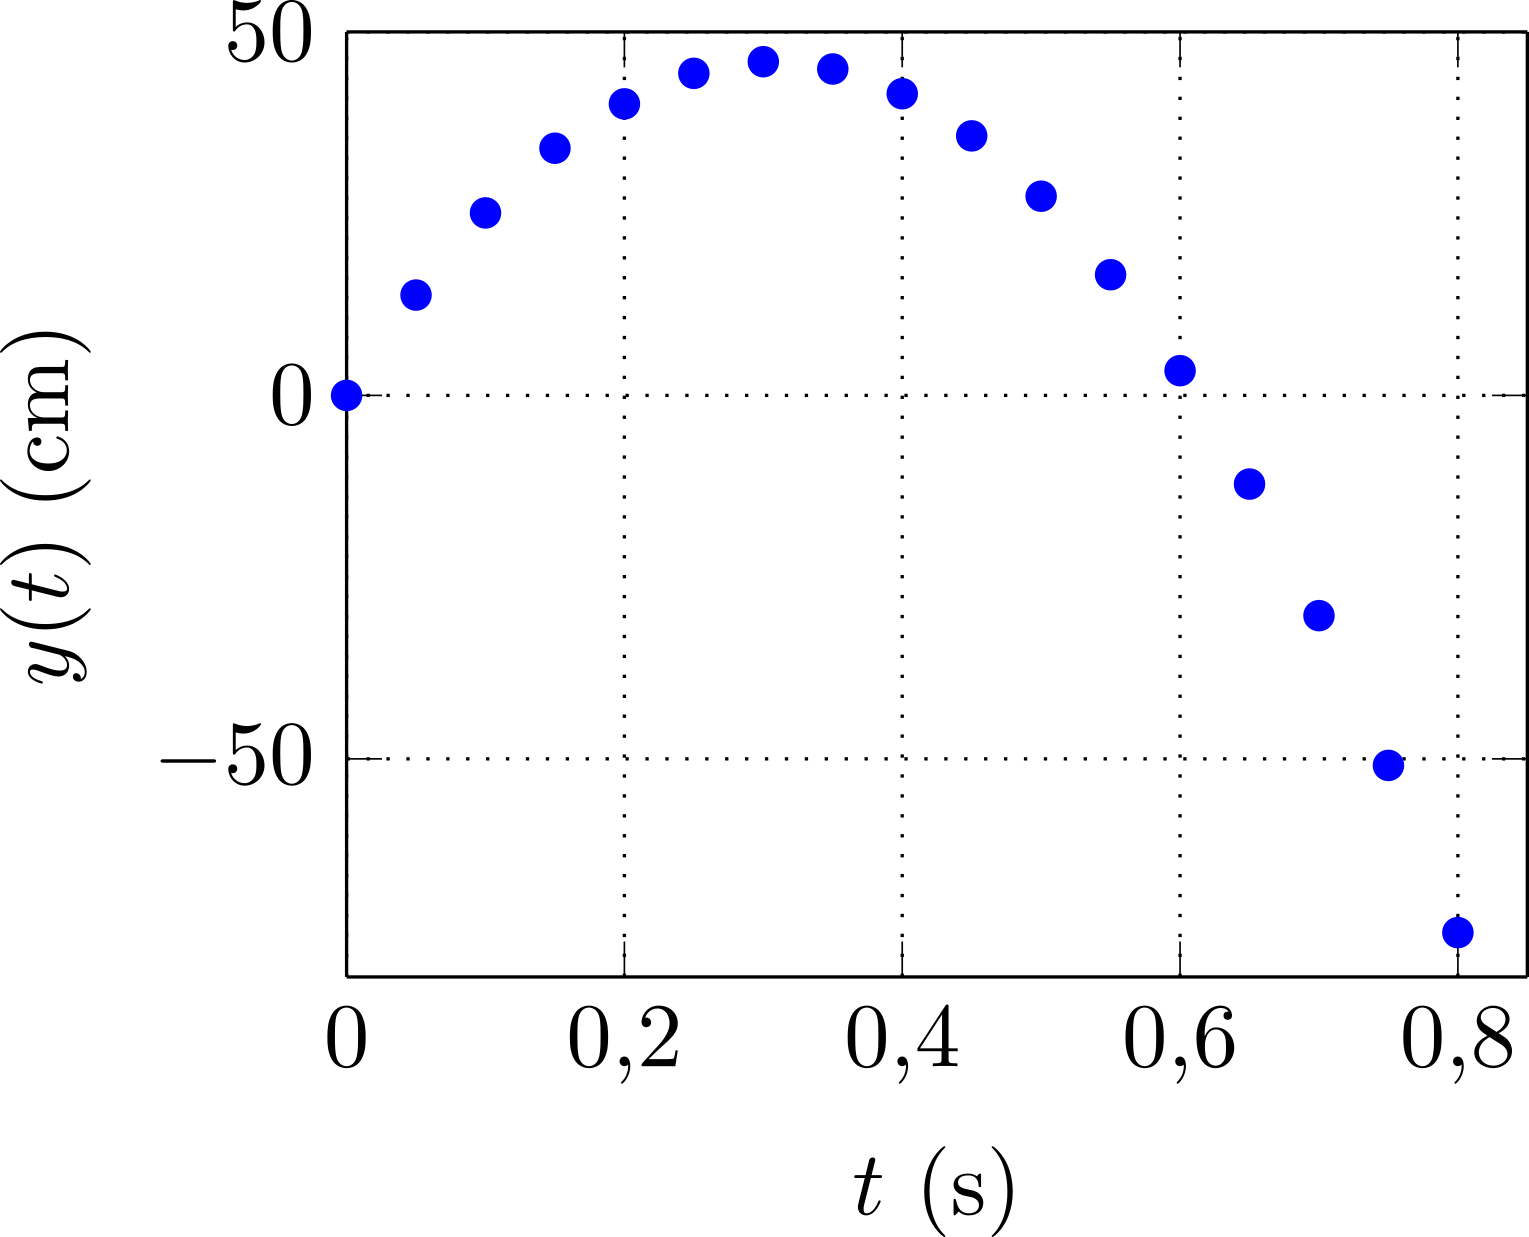
\includegraphics[width=\linewidth]{y_vo}
    \end{center}
\end{minipage}

% \begin{itemize}
%     \item chute dans le glycérol~: \smallbreak
%         \hfill
%         \begin{minipage}{0.35\linewidth}
%             \begin{center}
%                 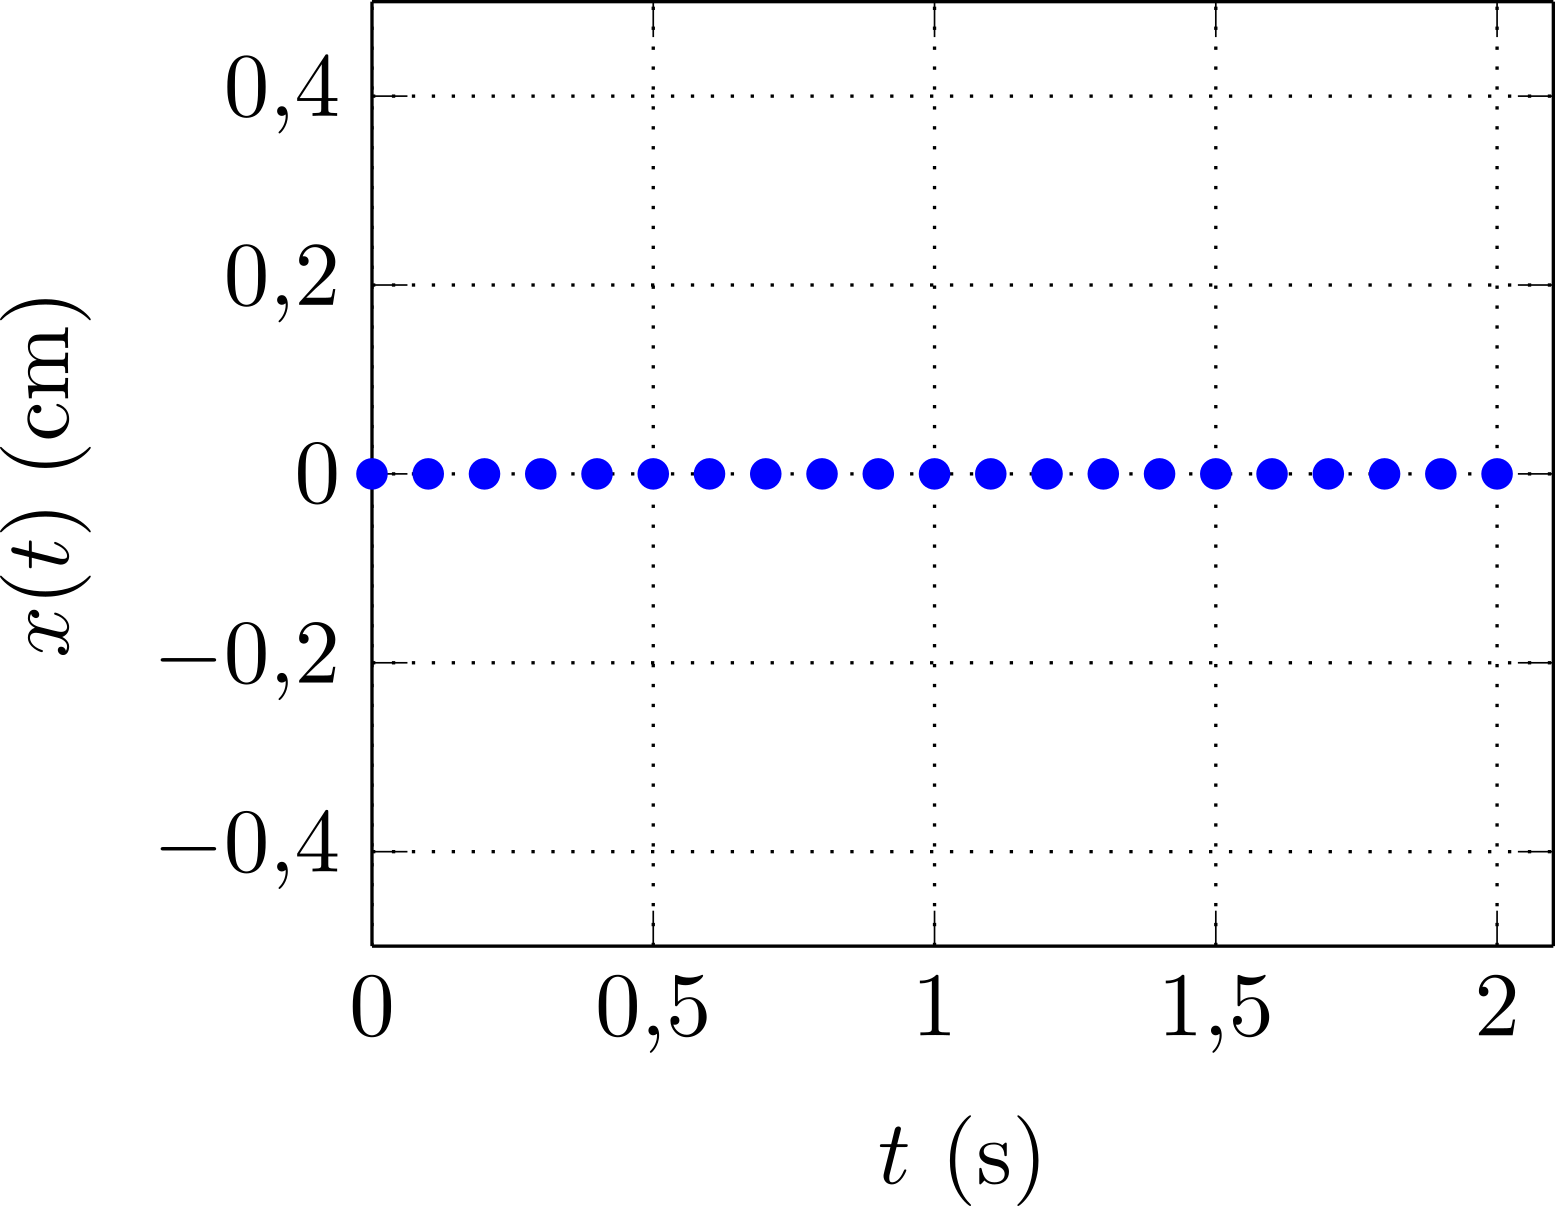
\includegraphics[width=\linewidth]{x_glyc}
%             \end{center}
%         \end{minipage}
%         \begin{minipage}{0.35\linewidth}
%             \begin{center}
%                 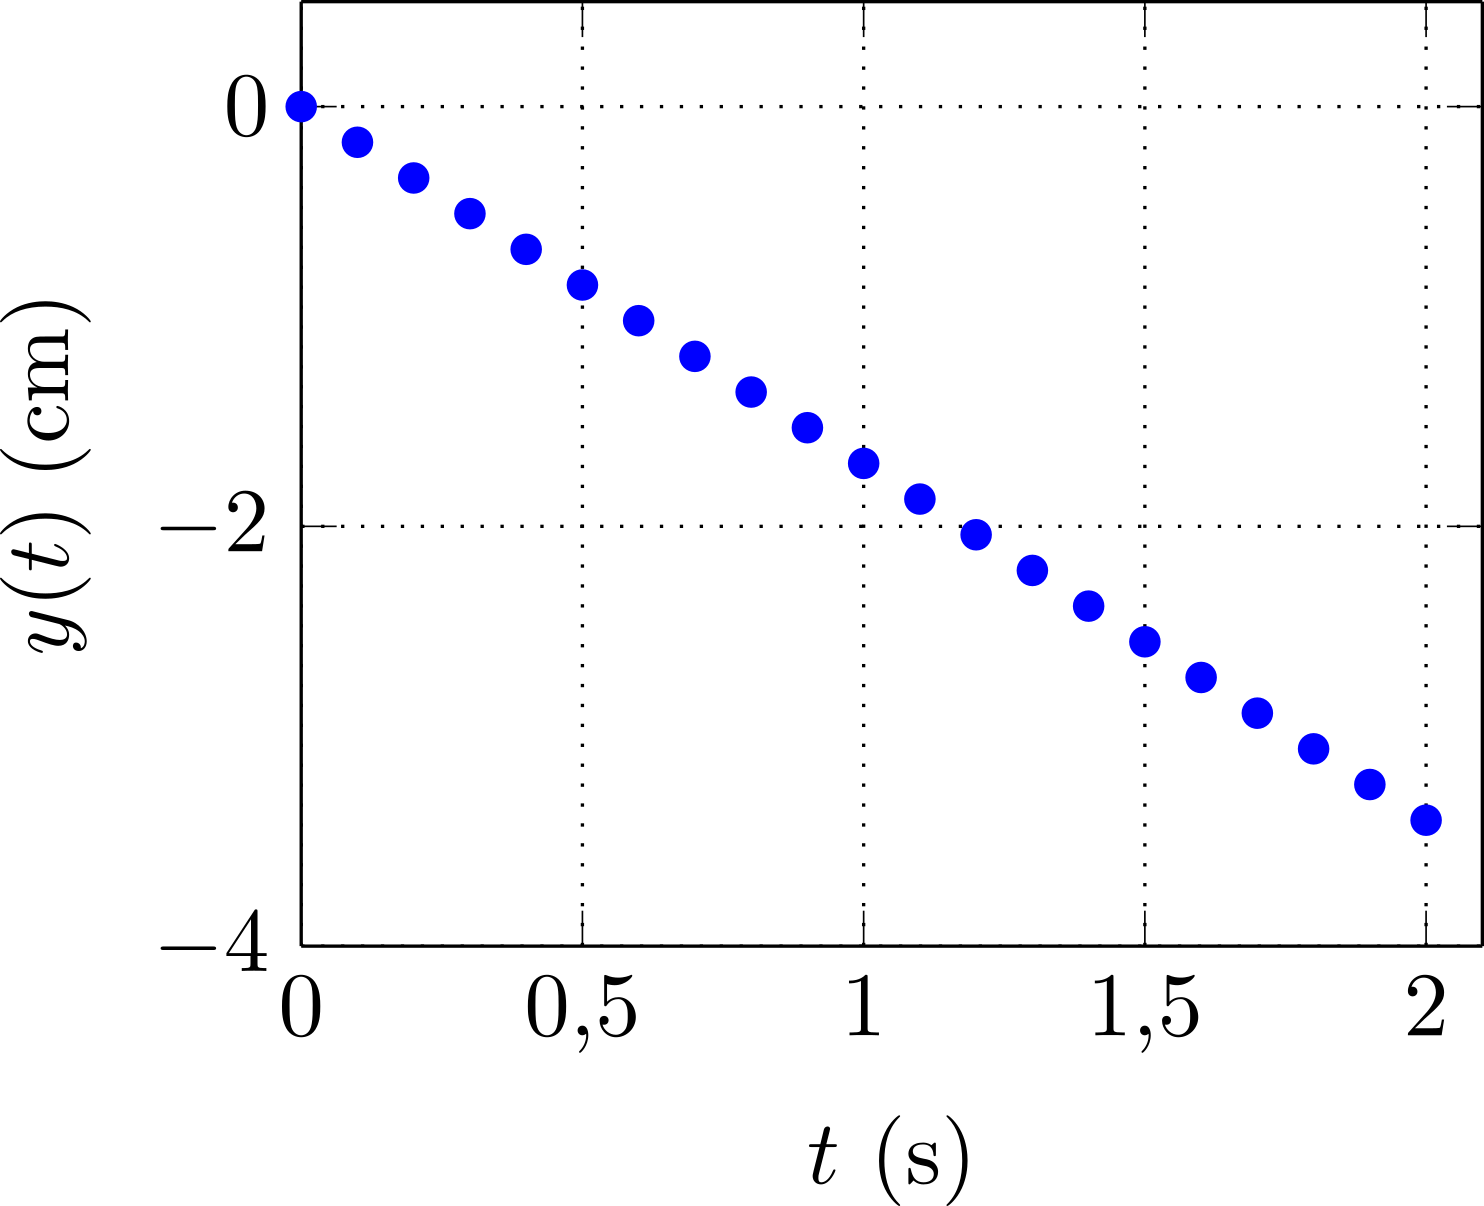
\includegraphics[width=\linewidth]{y_glyc}
%             \end{center}
%         \end{minipage}
%         \hfill~
%     \item chute libre sans vitesse initiale~: \smallbreak
%         \hfill
%         \begin{minipage}{0.35\linewidth}
%             \begin{center}
%                 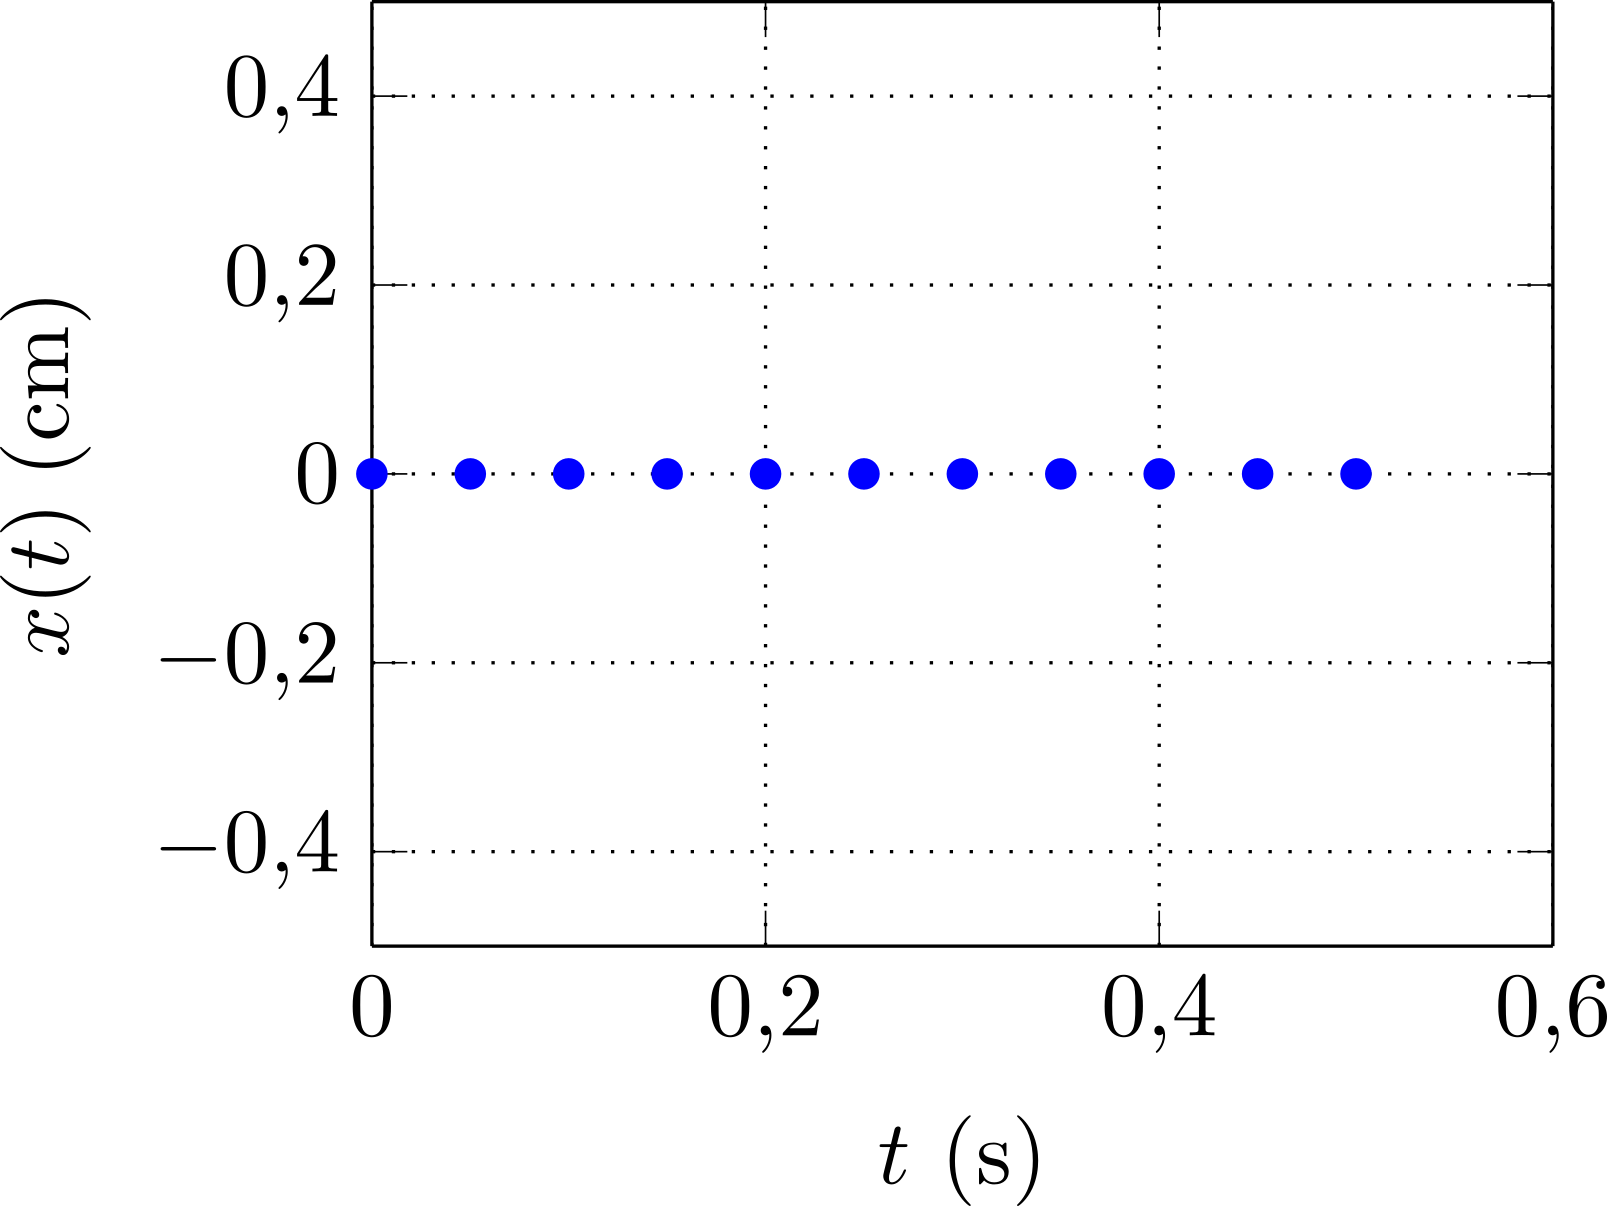
\includegraphics[width=\linewidth]{x_nov}
%             \end{center}
%         \end{minipage}
%         \begin{minipage}{0.35\linewidth}
%             \begin{center}
%                 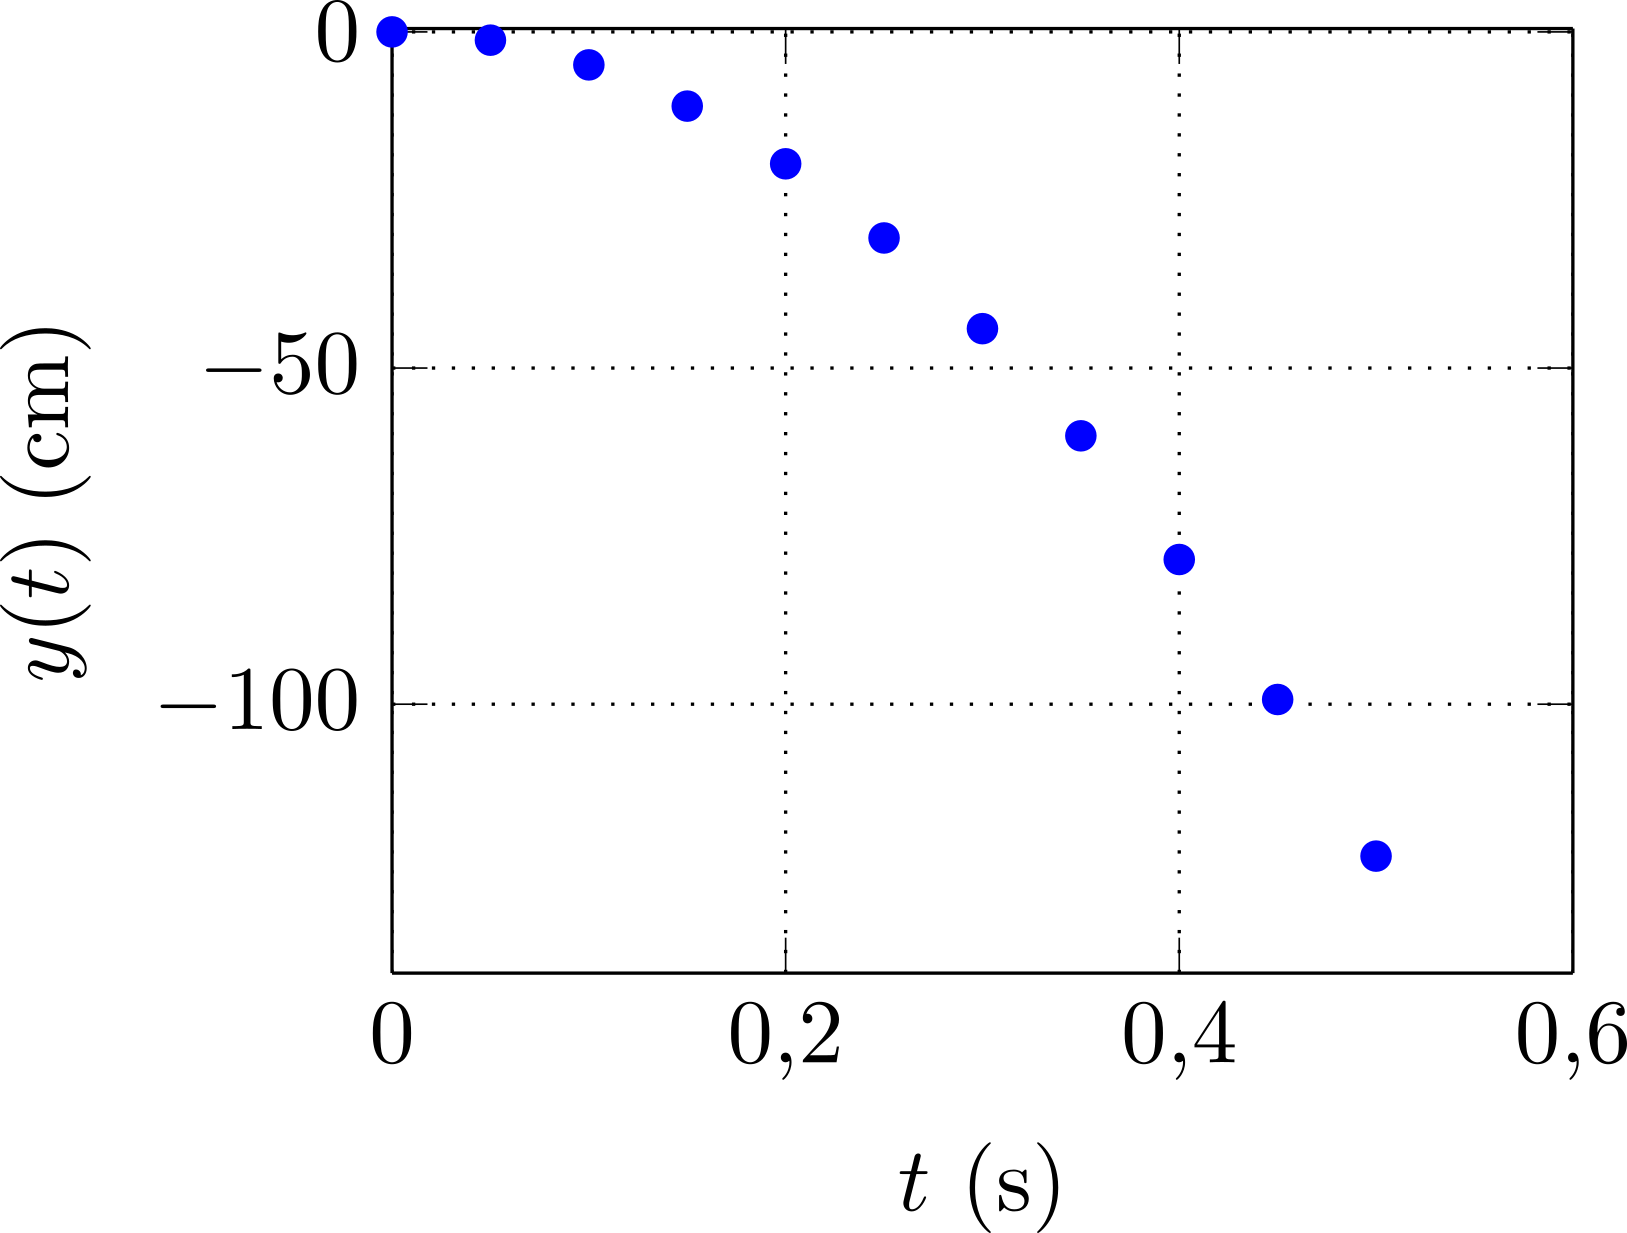
\includegraphics[width=\linewidth]{y_nov}
%             \end{center}
%         \end{minipage}
%         \hfill~
%     \item chute libre avec vitesse initiale~: \smallbreak
%         \hfill
%         \begin{minipage}{0.35\linewidth}
%             \begin{center}
%                 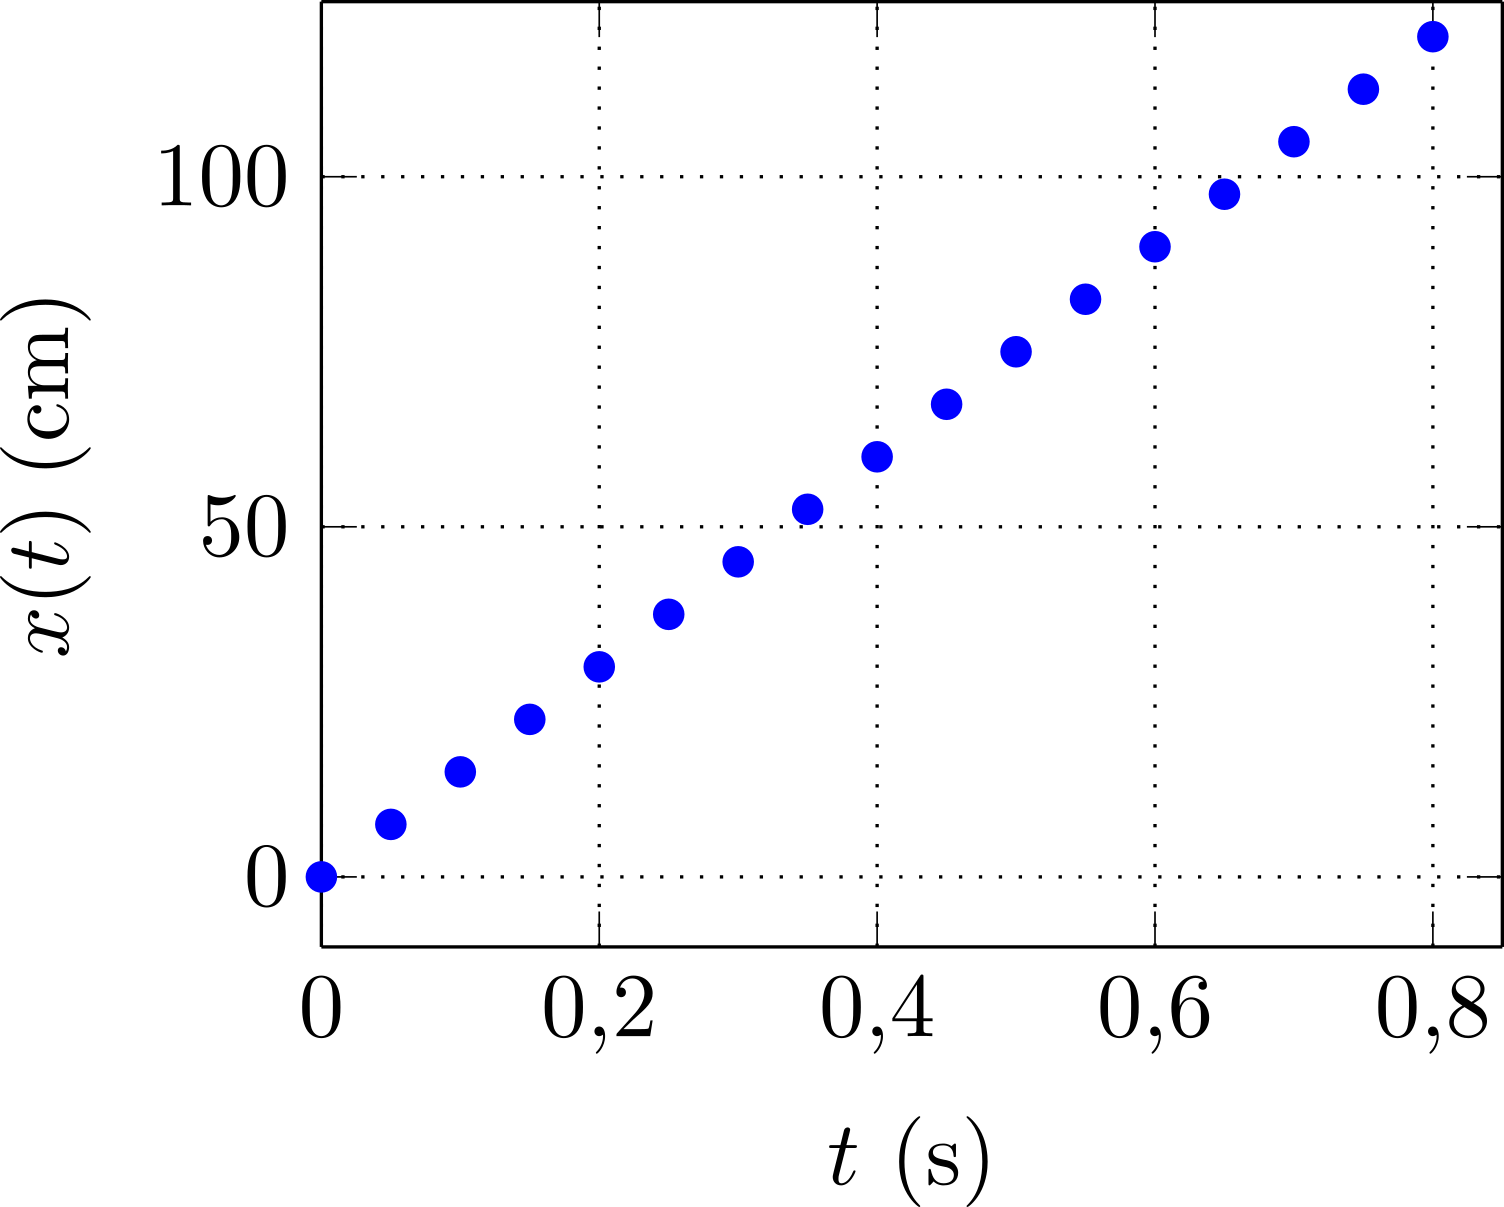
\includegraphics[width=\linewidth]{x_vo}
%             \end{center}
%         \end{minipage}
%         \begin{minipage}{0.35\linewidth}
%             \begin{center}
%                 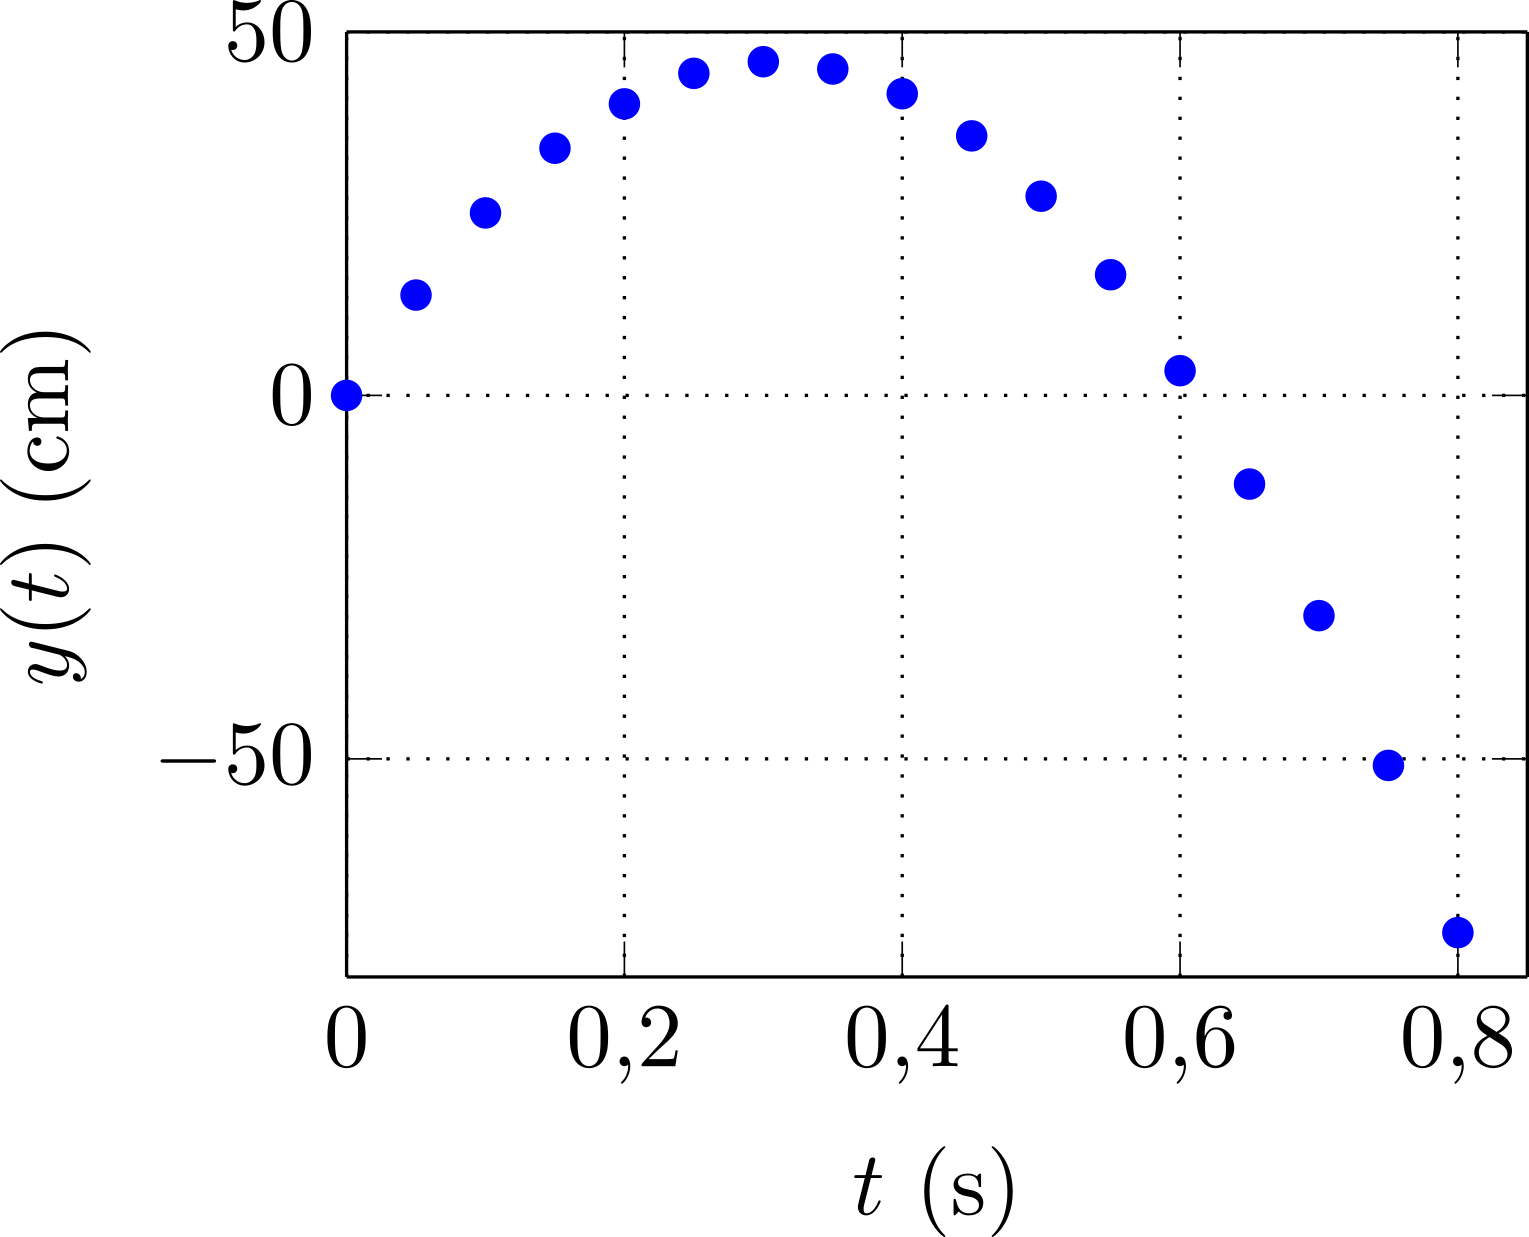
\includegraphics[width=\linewidth]{y_vo}
%             \end{center}
%         \end{minipage}
%         \hfill~
% \end{itemize}

% Les équations horaries peuvent aussi être des expressions analytiques de $x(t)$,
% $y(t)$ et $z(t)$ obtenues à partir d'une modélisation du problème.

\begin{rdefi}{Déf.}
    La \textbf{trajectoire} est l'ensemble des positions successives du point M
    au cours du temps. C'est le «~dessin~» fait par le mobile au cours du temps.
\end{rdefi}

Sur les exemples précédents, la trajectoire est la courbe $y(x)$ car le
mouvement est plan. C'est une droite dans les deux premiers cas, et une parabole
dans le dernier. \bigbreak

\begin{minipage}{0.31\linewidth}
    \begin{center}
        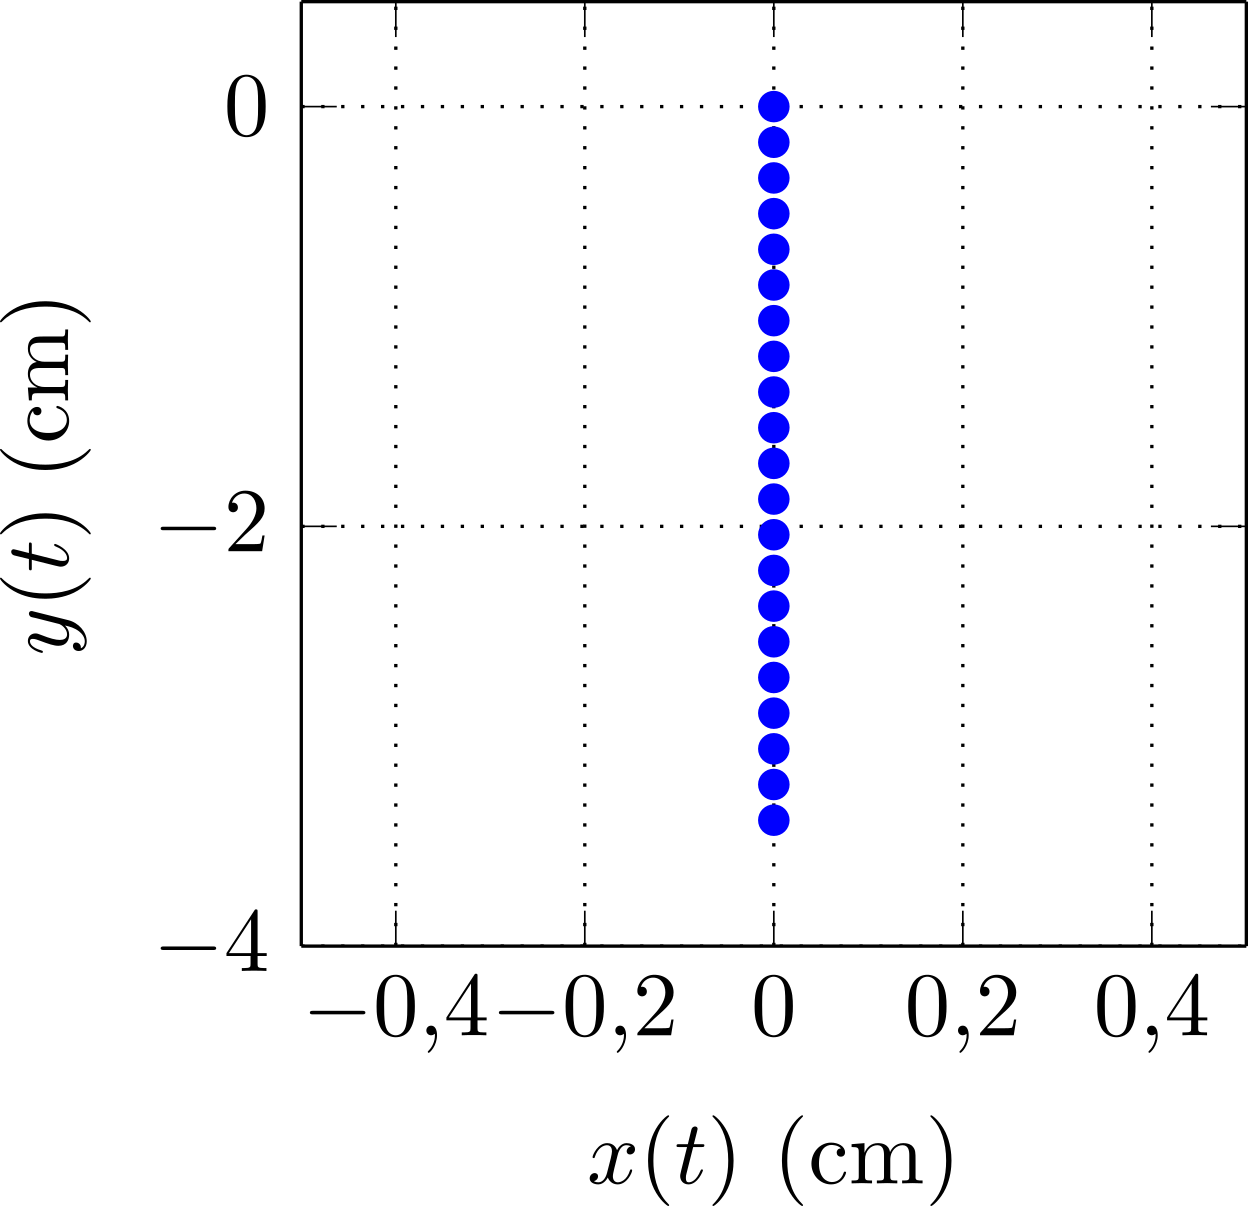
\includegraphics[width=\linewidth]{traj_glyc}
    \end{center}
\end{minipage}
\hfill
\begin{minipage}{0.31\linewidth}
    \begin{center}
        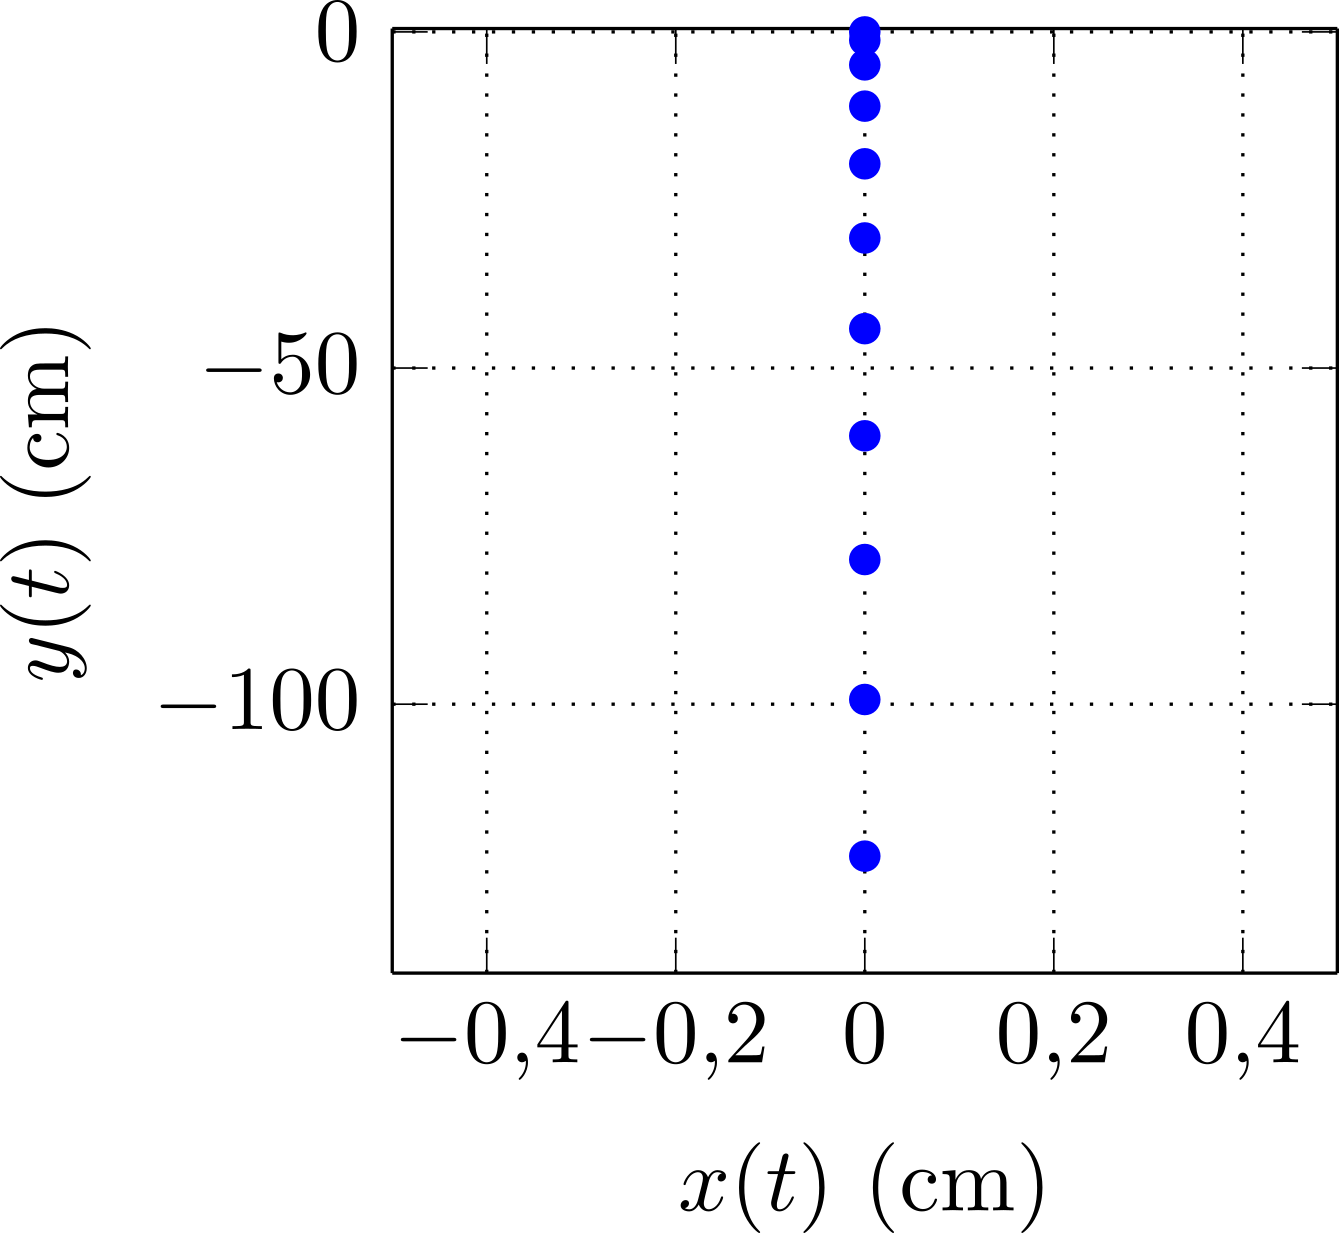
\includegraphics[width=\linewidth]{traj_nov}
    \end{center}
\end{minipage}
\hfill
\begin{minipage}{0.31\linewidth}
    \begin{center}
        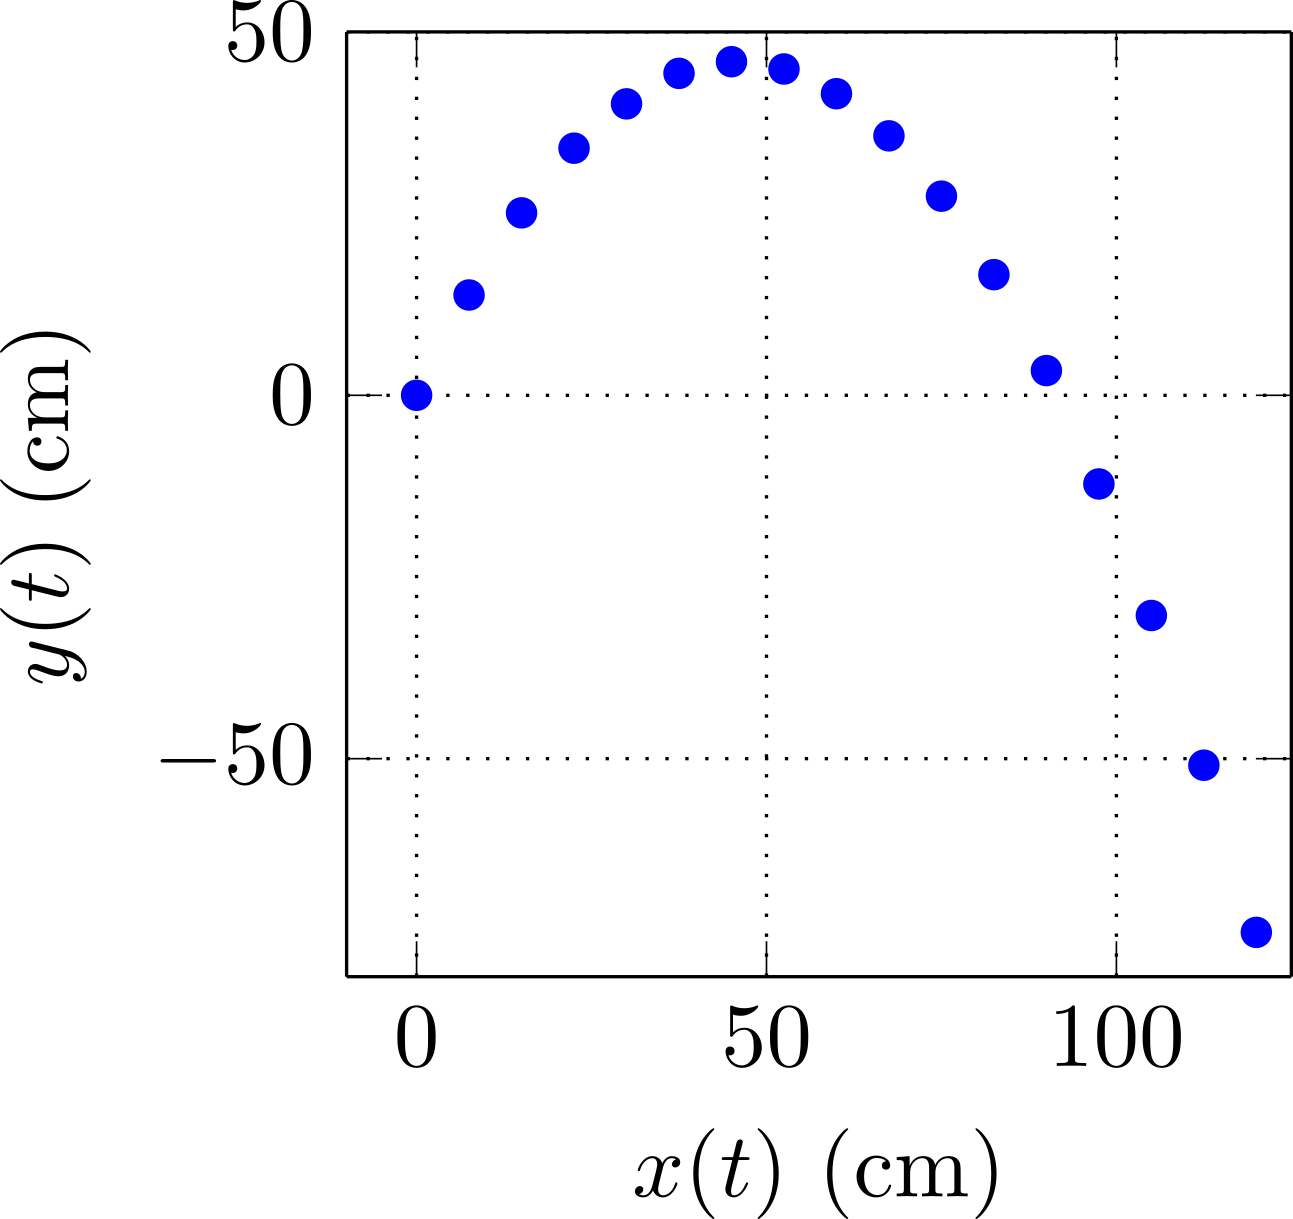
\includegraphics[width=\linewidth]{traj_vo}
    \end{center}
\end{minipage}

\vspace{-10pt}
\subsection{Vitesse}
\begin{bdefi}{Définitions}
    \begin{minipage}{0.70\linewidth}
        On définit la \textbf{vitesse} comme le \textbf{taux d'accroissement} du
        vecteur position~:
        \[\cswitch{white}{\boxed{\vf(t) = \frac{\OM(t+\Dt) - \OM(t)}{\Dt}}}
        \qdonc
        [\vf] = \si{m.s^{-1}}\]
        Si on effectue des mesures très rapprochées, c'est-à-dire $\Dt \rightarrow
        0$, on définit alors la vitesse \textit{instantanée} comme étant la
        \textit{dérivée} du vecteur position~:
        \[\cswitch{white}{\boxed{\vf(t) = \dv{\OM(t)}{t}}}\]
    \end{minipage}
    \hfill
    \begin{minipage}{0.29\linewidth}
        \begin{center}
            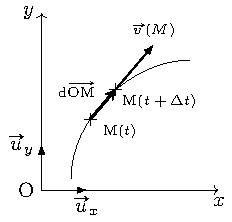
\includegraphics[width=\linewidth]{vec_vit}
        \end{center}
    \end{minipage}
\end{bdefi}

Ainsi, si le vecteur position est
\[\OM(t) = x(t)\ux + y(t)\uy + z(t)\uz\]
alors
\[\vf(t) = \dv{t}(x(t)\ux + y(t)\uy + z(t)\uz)\]
Or, \textbf{en coordonnées cartésiennes}, les vecteurs de base ne varient pas
avec le temps~: il ne changent pas de direction et restent unitaires. On peut
donc les considérer comme des constantes multiplicatives, et ainsi
\[\cswitch{white}{\vf(t) = \dv{x}{t}(t)\ux + \dv{y}{t}(t)\uy + \dv{z}{t}(t)\uz}\]
Pour alléger l'écriture, on introduit une notation~:
\begin{rdefi}{Notation}
    En mécanique, les dérivées \textbf{par rapport au temps} se notent avec un
    point sur la fonction~:
    \[\dv{x}{t}(t) = \xp(t)\]
\end{rdefi}
Ainsi, on trouve
\[\cswitch{white}{\boxed{\vf(t) = \xp(t)\ux + \yp(t)\uy + \zp(t)\uz}}\]

\begin{rexem}{Exemple}
    En reprenant les exemples précédents~:
    \begin{itemize}
        \item Pour la chute dans le glycérol, $\xp = 0$ et $\yp = \cte$. Ainsi,
            $\vf$ est constant, et dirigé vers le bas.
        \item Pour la chute libre sans vitesse initiale, $\xp = 0$ et $\yp$
            diminue linéairement~: le vecteur vitesse est variable, dirigé vers
            le bas.
        \item Pour la chute libre avec vitesse initiale, $\xp = \cte$ et $\yp$
            diminue linéairement~: le vecteur vitesse est variable et change de
            direction.
    \end{itemize}
\end{rexem}

\begin{bimpo}{\includehand{-90}{0.8cm}}
    Selon le contexte, on fera particulièrement attention à ne pas confondre le
    mot «~vitesse~» avec le \textbf{vecteur} ou avec sa \textbf{norme}. Une
    vitesse, en norme, ne saurait être négative~; un vecteur vitesse peut être
    négatif.
\end{bimpo}

\subsection{Accélération}
L'accélération est la grandeur physique qui mesure la variation de la vitesse.
\begin{bdefi}{Définitions}
    On définit l'\textbf{accélération} comme le \textbf{taux d'accroissement} du
    vecteur vitesse~:
    \[\cswitch{white}{\boxed{\af(t) = \frac{\vf(t+\Dt) - \vf(t)}{\Dt}}}
    \qdonc
    [\af] = \si{m.s^{-2}}\]
    Si on effectue des mesures très rapprochées, c'est-à-dire $\Dt \rightarrow
    0$, on définit alors l'accélération \textit{instantanée} comme étant la
    \textit{dérivée} du vecteur vitesse, et dérivée seconde de la position~:
    \[\cswitch{white}{\boxed{\af(t) = \dv{\vf(t)}{t}}}
    \qet
    \cswitch{white}{\boxed{\af(t) = \dv[2]{\OM(t)}{t}}}\]
\end{bdefi}

Par distribution de l'opérateur $\dv{t}$, on obtient
\[\cswitch{white}{\boxed{\af(t) = \xpp(t)\ux + \ypp(t)\uy + \zpp(t)\uz}}\]

\begin{rexem}{Exemple}
    En reprenant les exemples précédents~:
    \begin{itemize}
        \item Pour la chute dans le glycérol, $\xpp$ et $\ypp$ sont nuls~: le
            vecteur accélération est nul.
        \item Pour la chute libre sans vitesse initiale, $\xpp = 0$ et $\ypp$
            est constant~: le vecteur accélération est constant, dirigé vers le
            bas.
        \item Pour la chute libre avec vitesse initiale, $\xpp = 0$ et $\ypp$
            est constant~: le vecteur accélération est constant, dirigé vers le
            bas.
    \end{itemize}
\end{rexem}

\begin{bimpo}{\includehand{-90}{0.8cm}}
    Une accélération peut être négative ou nulle~:
    \begin{itemize}
        \item En physique l'accélération est liée à la \textbf{variation du
            vecteur vitesse}, souvent différent de l'utilisation courante de ce
            mot.
        \item Pour que l'accélération soit nulle, il faut que toutes les
            composantes de la vitesse ne varient pas. Un mouvement peut être à
            vitesse constante en norme, mais d'accélération non nulle.
    \end{itemize}
\end{bimpo}

\section{Exemples de mouvements}
\subsection{Rappel mathématique}
\begin{rrapp}{Rappel}
    \begin{itemize}
        \item Si $\xp(t) = 0$, alors $x(t) = x_0$ avec $x_0 = \cte$.
        \item Si $\xp(t) = v_0$, alors $x(t) = v_0t + x_0$ avec $x_0 = \cte$.
        \item Si $\xp(t) = a_0t$, alors $x(t) = \DS \frac{1}{2}a_0t^2 +  x_0$
            avec $x_0 = \cte$.
    \end{itemize}
\end{rrapp}

\subsection{Mouvement rectiligne uniforme}
\begin{rdefi}{Déf.}
    Un mouvement est dit \textit{rectiligne uniforme} si le vecteur vitesse est
    constant.
\end{rdefi}
Par exemple,
\[\vf = v_0\ux\]
donne un mouvement rectiligne uniforme. C'est le cas de la chute dans le
glycérol. Dans ce cas,
\cswitch{white}{
\[
    \left\{
        \begin{array}{l}
            \xp(t) = v_0\\
            \yp(t) = 0\\
            \zp(t) = 0
        \end{array}
    \right.
    \Longrightarrow
    \left\{
        \begin{array}{l}
            x(t) = v_0t + x_0\\
            y(t) = y_0\\
            z(t) = z_0
        \end{array}
    \right.
\]}
avec $x_0$, $y_0$ et $z_0$ des constantes que l'on peut calculer à l'aide des
conditions initiales.

\subsection{Mouvement rectiligne uniformément accéléré}
\begin{rdefi}{Déf.}
    Un mouvement est dit rectiligne \textit{uniformément accéléré} si le vecteur
    \textbf{accélération} est constant et que le mouvement s'effectue en ligne
    droite.
\end{rdefi}
Par exemple,
\[\af = -g\uy\]
avec des conditions initiales nulles donne un mouvement rectiligne uniformément
accéléré. C'est le cas de la chute libre sans vitesse initiale. Contextualisons
l'étude~: \smallbreak
\begin{minipage}{0.80\linewidth}
    \begin{itemize}
        \item \textbf{Système}~:\cswitch{white}{point matériel.}
        \item \textbf{Référentiel}~:\cswitch{white}{celui du laboratoire.}
        \item \textbf{Repère}~:\cswitch{white}{cartésien avec $\uy$ verticale
            ascendante.}
        \item \textbf{Origine des temps}~:\cswitch{white}{le moment où la balle
            est lâchée, tel que $\vf(0) = \of$.}
        \item \textbf{Origine du repère}~:\cswitch{white}{O tel que $\OM(0) =
            \of$.}
    \end{itemize}
\end{minipage}
\hfill
\begin{minipage}{0.19\linewidth}
    \begin{center}
        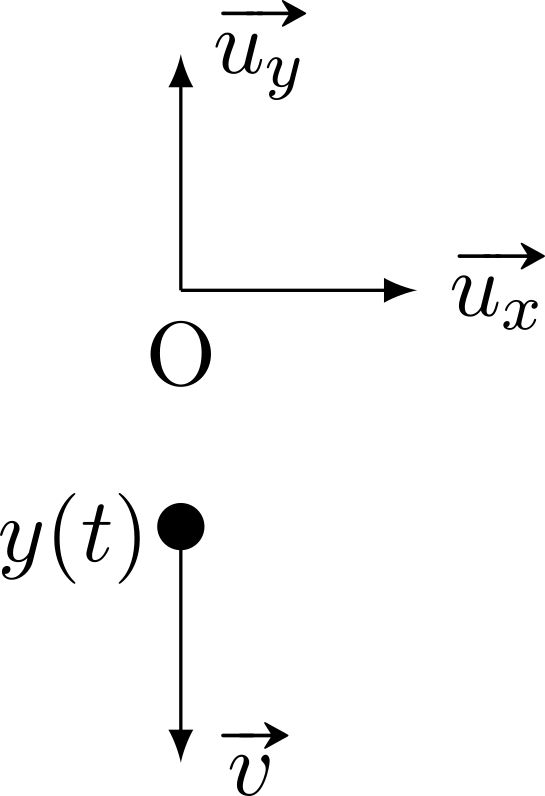
\includegraphics[height=3cm]{nov_init}
    \end{center}
\end{minipage}

Par définition,
\[\cswitch{white}{\af(t) = \xpp(t)\ux + \ypp(t)\uy + \zpp(t)\uz}\]
Soit
\[
\cswitch{white}{
    \left\{
        \begin{array}{l}
            \xpp(t) = 0\\
            \ypp(t) = -g\\
            \zpp(t) = 0
        \end{array}
    \right.
    \Longrightarrow
    \left\{
        \begin{array}{l}
            \xp(t) = v_{x,0}\\
            \yp(t) = -gt + v_{y,0}\\
            \zp(t) = v_{z,0}
        \end{array}
    \right.
}\]
Or,
\[\cswitch{white}{
    \vf(0) = \of
    \qdonc
    \left\{
        \begin{array}{l}
            \xp(0) = v_{x,0} = 0\\
            \yp(0) = v_{y,0} = 0\\
            \zp(0) = v_{z,0} = 0
        \end{array}
    \right.
}\]
Ainsi
\[
\cswitch{white}{
    \left\{
        \begin{array}{l}
            \xp(t) = 0\\
            \yp(t) = -gt\\
            \zp(t) = 0
        \end{array}
    \right.
    \Longrightarrow
    \left\{
        \begin{array}{l}
            x(t) = x_{0}\\
            y(t) = -\dfrac{1}{2}gt^2 + y_{0}\\
            z(t) = z_{0}
        \end{array}
    \right.
}\]
Seulement,
\[\cswitch{white}{
    \OM(0) = \of
    \qdonc
    \left\{
        \begin{array}{l}
            x(0) = y_{0} = 0\\
            y(0) = y_{0} = 0\\
            z(0) = z_{0} = 0
        \end{array}
    \right.
}\]
Autrement dit,
\[\cswitch{white}{
    \boxed{
    \left\{
        \begin{array}{l}
            x(t) = 0\\
            y(t) = -\dfrac{1}{2}gt^2\\
            z(t) = 0
        \end{array}
    \right.
}}\]
Ce sont les équations horaires du mouvement, décrivant une droite dans l'espace.

\hfill
\begin{minipage}{0.45\linewidth}
    \begin{center}
        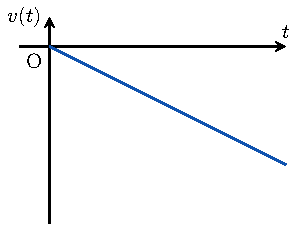
\includegraphics[width=6.5cm]{nov_vy}
    \end{center}
    \captionof{figure}{Évolution de $v_y$ avec le temps.}
\end{minipage}
\hfill
\begin{minipage}{0.45\linewidth}
    \begin{center}
        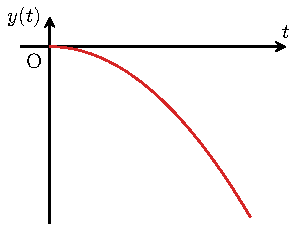
\includegraphics[width=6.5cm]{nov_y}
    \end{center}
    \captionof{figure}{Évolution de $y$ avec le temps.}
\end{minipage}
\hfill~

\subsection{Mouvement courbe uniformément accéléré}
\begin{minipage}{0.75\linewidth}
    En reprenant la même situation que ci-dessus mais avec des conditions
    initiales non nulles, on trouvera un mouvement courbe. Prenons
    \[\vf(0) = v_0\ux\]
    avec $v_0 \neq 0$. On garde $\af = -g \uy$, le même repère et la même
    origine~: $\OM(0) = 0$. Par définition,
\end{minipage}
\hfill
\begin{minipage}{0.23\linewidth}
    \begin{center}
        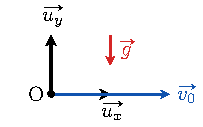
\includegraphics[width=\linewidth]{vo_init}
    \end{center}
\end{minipage}

\[\cswitch{white}{\af(t) = \xpp(t)\ux + \ypp(t)\uy + \zpp(t)\uz}\]
Soit
\[
\cswitch{white}{
    \left\{
        \begin{array}{l}
            \xpp(t) = 0\\
            \ypp(t) = -g\\
            \zpp(t) = 0
        \end{array}
    \right.
    \Longrightarrow
    \left\{
        \begin{array}{l}
            \xp(t) = v_{x,0}\\
            \yp(t) = -gt + v_{y,0}\\
            \zp(t) = v_{z,0}
        \end{array}
    \right.
}\]
Or,
\[\cswitch{white}{
    \vf(0) = v_0\ux
    \qdonc
    \left\{
        \begin{array}{l}
            \xp(0) = v_{x,0} = v_0\\
            \yp(0) = v_{y,0} = 0\\
            \zp(0) = v_{z,0} = 0
        \end{array}
    \right.
}\]
Ainsi
\[
\cswitch{white}{
    \left\{
        \begin{array}{l}
            \xp(t) = v_0\\
            \yp(t) = -gt\\
            \zp(t) = 0
        \end{array}
    \right.
    \Longrightarrow
    \left\{
        \begin{array}{l}
            x(t) = v_0t + x_{0}\\
            y(t) = -\dfrac{1}{2}gt^2 + y_{0}\\
            z(t) = z_{0}
        \end{array}
    \right.
}\]
Seulement,
\[\cswitch{white}{
    \OM(0) = \of
    \qdonc
    \left\{
        \begin{array}{l}
            x(0) = y_{0} = 0\\
            y(0) = y_{0} = 0\\
            z(0) = z_{0} = 0
        \end{array}
    \right.
}\]
Autrement dit,
\[\cswitch{white}{
    \boxed{
    \left\{
        \begin{array}{l}
            x(t) = v_0t\\
            y(t) = -\dfrac{1}{2}gt^2\\
            z(t) = 0
        \end{array}
    \right.
}}\]

\begin{minipage}{0.48\linewidth}
    \begin{center}
        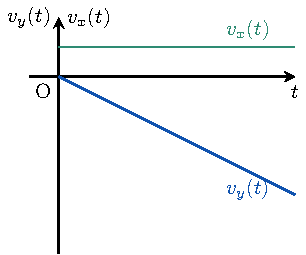
\includegraphics[width=\linewidth]{vo_vv}
    \end{center}
    \captionof{figure}{Évolution des vitesses avec le temps.}
\end{minipage}
\hfill
\begin{minipage}{0.48\linewidth}
    \begin{center}
        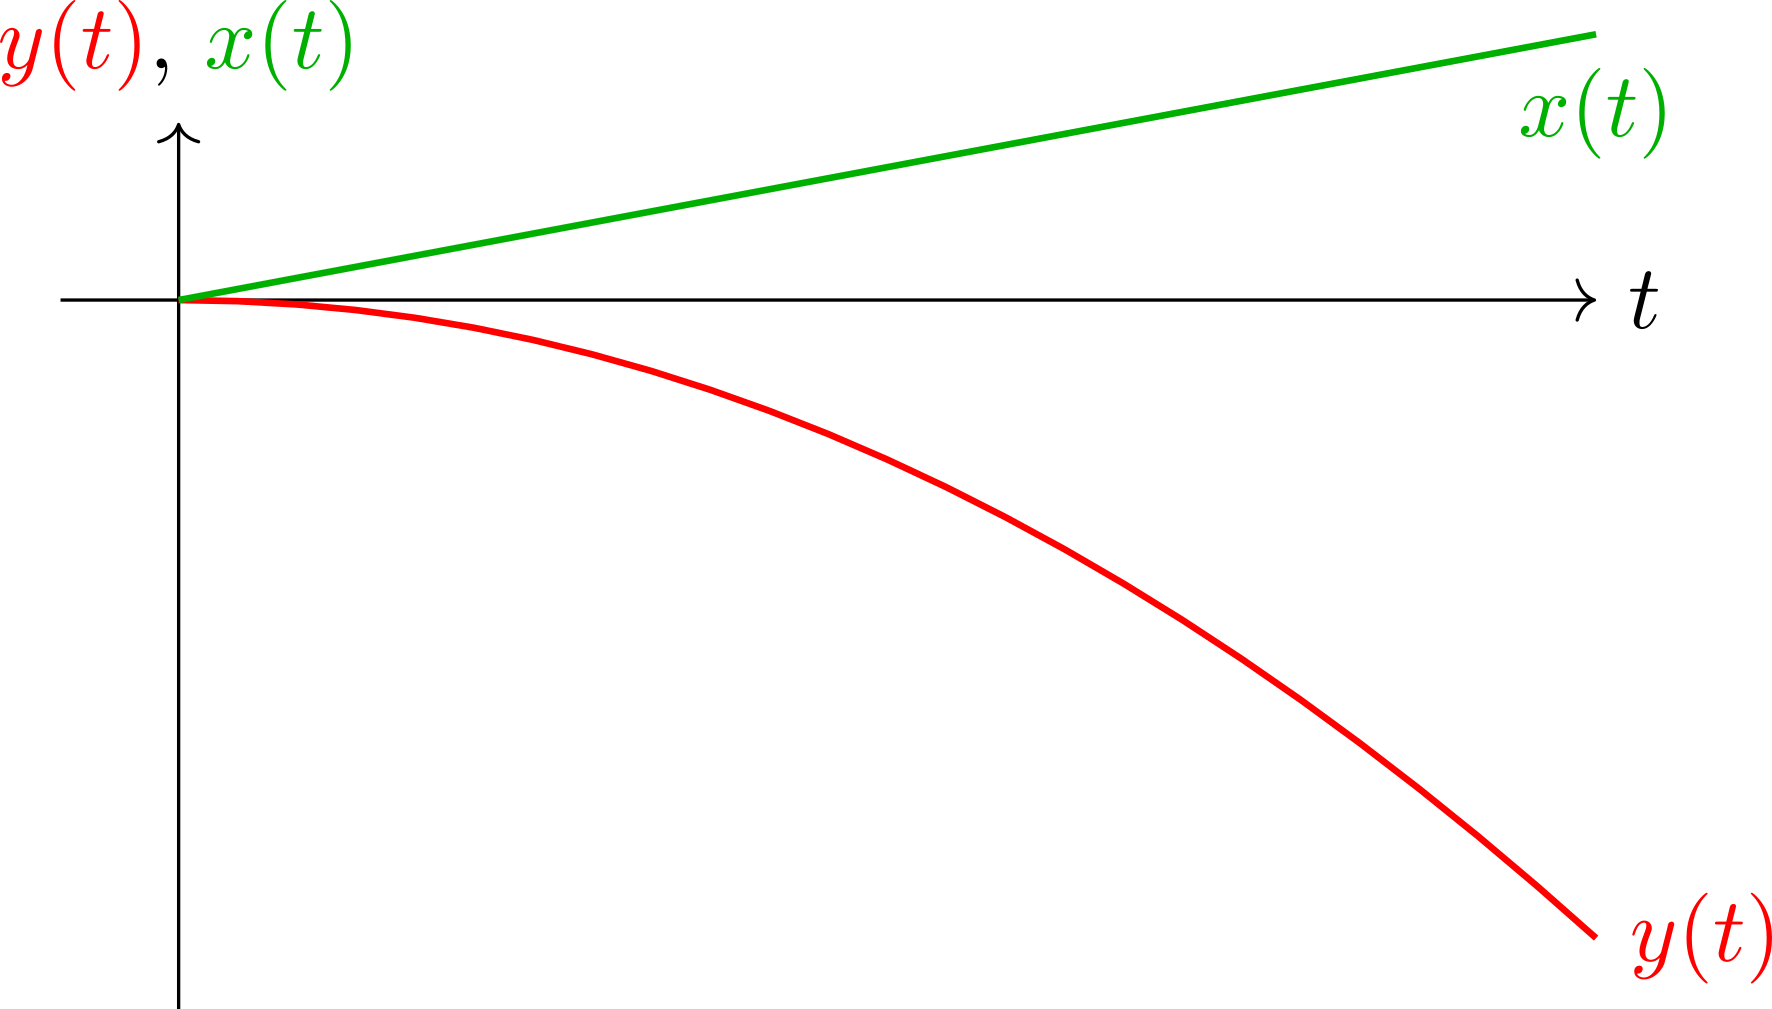
\includegraphics[width=\linewidth]{vo_xx}
    \end{center}
    \captionof{figure}{Évolution des positions avec le temps.}
\end{minipage} \bigbreak

\begin{minipage}{0.60\linewidth}
    Pour obtenir la trajectoire, on veut déterminer la courbe $y(x)$ décrite dans le
    plan $xy$. Pour cela, exprimons $t$ en fonction de $x$ et remplaçons $t$ dans
    l'expression de $y$~:
    \begin{gather*}
        t = \frac{x}{v_0}\\
        \Rightarrow
        y(x) = - \frac{1}{2}g \left( \frac{x}{v_0} \right)^2
        \Leftrightarrow
        \boxed{y(x) = - \frac{g}{2v_0{}^2}x^2}
    \end{gather*}
    La trajectoire obtenue est alors une parabole.
\end{minipage}
\hfill
\begin{minipage}{0.35\linewidth}
    \begin{center}
        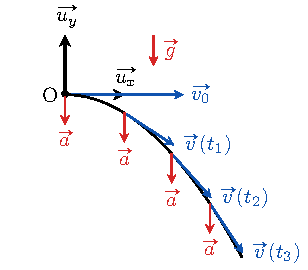
\includegraphics[width=\linewidth]{vo_traj}
    \end{center}
\end{minipage}

\end{document}
